\chapter[Marco Teórico]{Marco Teórico}
\label{cp:theoretical-framework}

\parindent0pt

% TODO: fix redaction of all sections, add references, and improve the connection between sections

Este capítulo presenta los fundamentos teóricos que sirven de base para este trabajo. Se aborda la estructura y funcionamiento de las cadenas de bloques, destacando sus características de descentralización, transparencia e inmutabilidad, así como los mecanismos de consenso que garantizan su seguridad y eficiencia. Además, se analiza el rol de los contratos inteligentes como herramientas para automatizar procesos y gestionar la lógica de negocio en entornos descentralizados. Asimismo, este capítulo explora los principios de la economía circular, enfatizando su enfoque regenerativo y su capacidad para transformar las cadenas de suministro hacia modelos más sostenibles. Se examinan las etapas del proceso de producción y reciclaje, con especial atención a la trazabilidad como habilitador para garantizar la transparencia y la eficiencia en una economía circular. Luego se incluye un análisis de la cadena de suministro del vidrio en el contexto mendocino, destacando su relevancia estratégica y los desafíos asociados a su implementación en un modelo circular. Finalmente, se explora el estado del arte de la tecnología \textit{blockchain} en la economía circular, identificando las tendencias actuales y las oportunidades de mejora en la trazabilidad y sostenibilidad de la cadena de suministro del vidrio.

\section{Blockchain}

La tecnología \textit{blockchain}, o cadena de bloques, sirve para registrar información digital de manera segura, transparente e inmutable. Es relevante comprender los motivos de su surgimiento como una tecnología disruptiva en los últimos años, antes de introducir su estructura y funcionamiento

Para entender la necesidad e impacto de la tecnología blockchain, primero es necesario analizar la arquitectura predominante de Internet hasta la actualidad, basada tradicionalmente en un modelo centralizado cliente-servidor. En este esquema, los datos son almacenados en servidores administrados por proveedores, quienes actúan como intermediarios de confianza entre los clientes o usuarios. Aunque este modelo ha facilitado el intercambio de información a escala masiva, también ha generado problemas de confianza, seguridad y privacidad. La centralización implica que los usuarios ceden el control y gestión de sus datos a terceros, lo que puede derivar en una dependencia significativa de estas entidades para la integridad y disponibilidad de la información. Ejemplos de esto incluyen la exposición de datos personales privados en ciber-ataques, la interrupción de servicios por fallas en servidores centrales o la censura de contenido por decisiones unilaterales de las plataformas \cite{pending}. Por ejemplo, cuando el servidor de Whatsapp deja de funcionar, los usuarios no pueden utilizar la aplicación para comunicarse hasta que el proveedor vuelva a hacerlo funcionar. Otro ejemplo, es cuando un proveedor sufre un ciber-ataque y se filtran contraseñas de los usuarios, quienes no tienen conocimiento de las vulnerabilidades que puede tener el proveedor, pero dependen de su servicio.

Ante los desafíos de confianza e integridad en los sistemas centralizados, la tecnología blockchain surgió en 2008 como una solución disruptiva. Su primera aplicación fue como base del sistema de criptomonedas Bitcoin \cite{satoshi2008bitcoin}, pero rápidamente demostró potencial por fuera del ámbito financiero. En la actualidad, blockchain se considera una herramienta útil para resolver problemas de confianza, transparencia e inmutabilidad en la gestión de datos. Su diseño permite registrar información de forma distribuida, sin necesidad de proveedores centralizados, habilitando la interacción directa entre múltiples partes \cite{bulkowska2023implementation}.

\begin{figure}[!htpb]
    \centering
    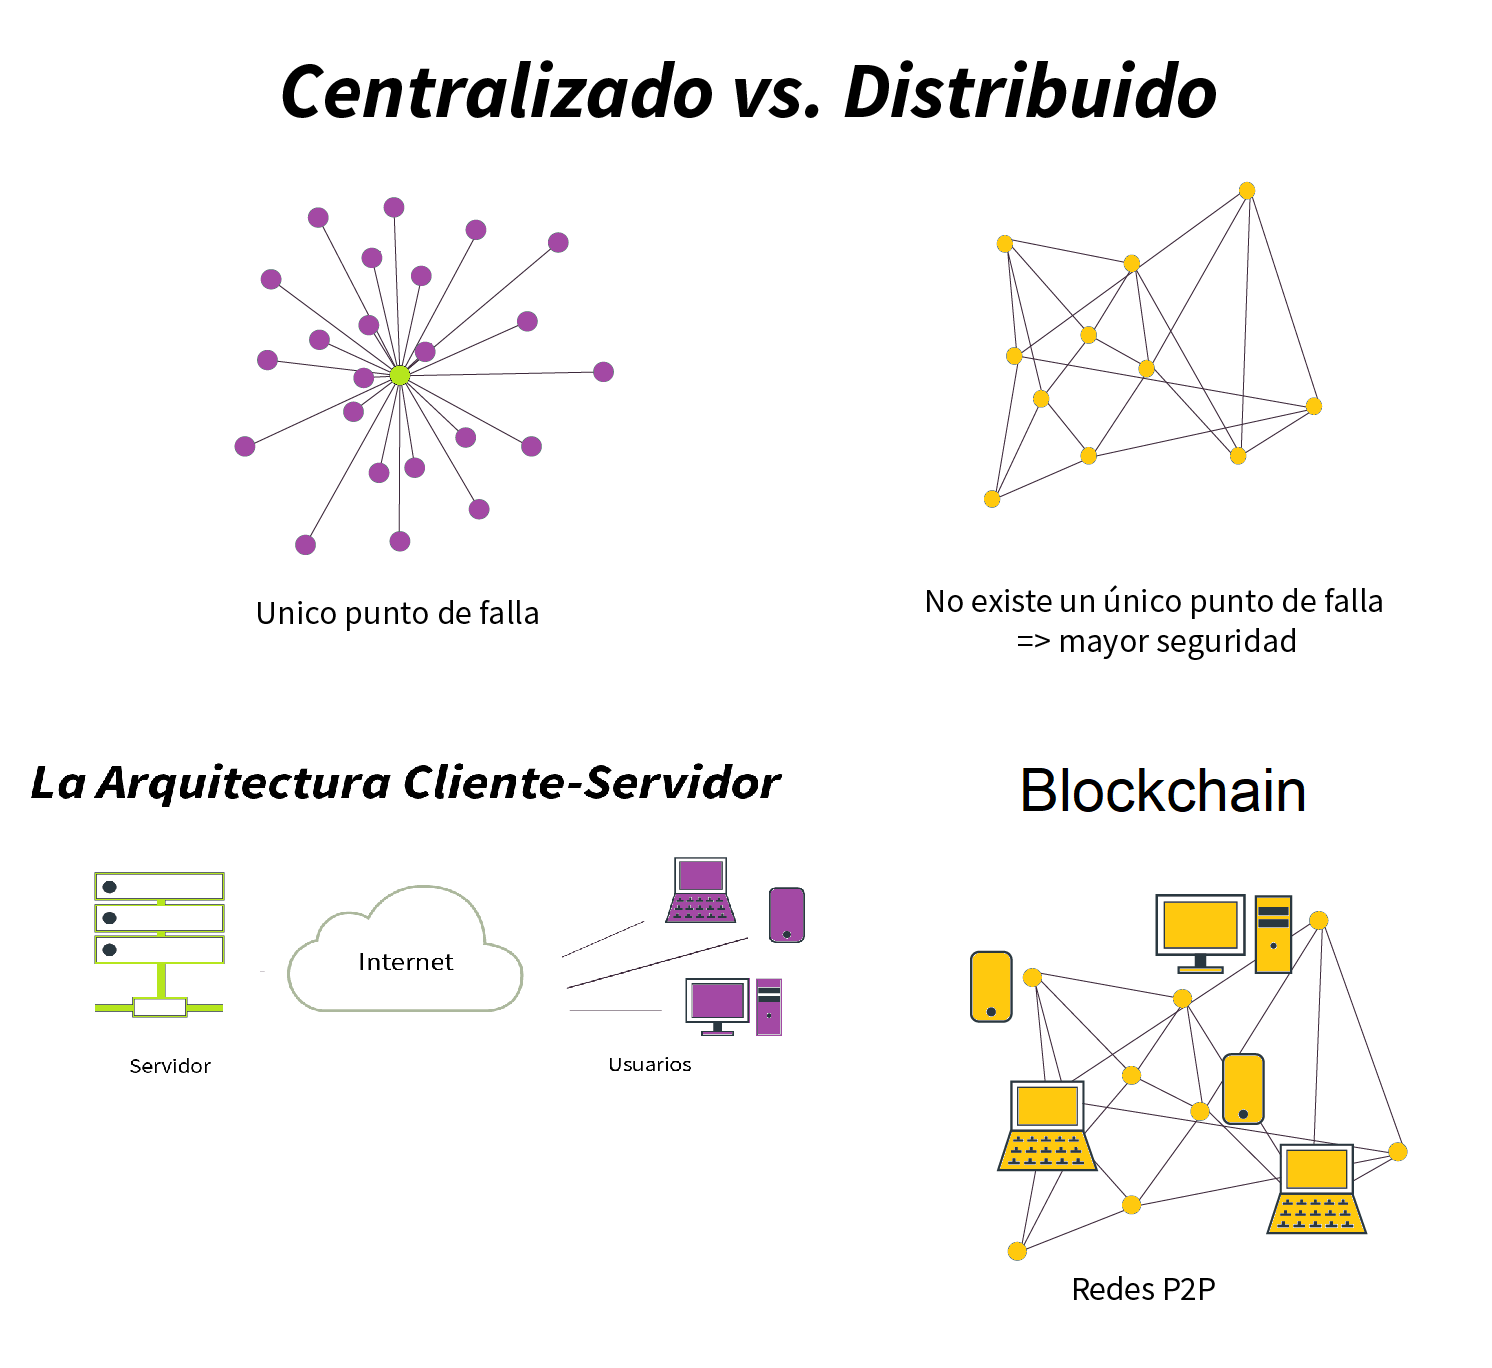
\includegraphics[width=0.8\textwidth]{Figures/cliente-server-vs-p2p.png}
    \caption{Comparación entre el modelo cliente-servidor y el modelo P2P}
    \label{fig:web-architecture}
\end{figure}

Es importante destacar que blockchain no introduce tecnologías completamente nuevas, sino que integra de forma innovadora principios existentes de la computación y las matemáticas. Combina conceptos de criptografía (para asegurar la información), redes distribuidas (para la replicación de los datos) y teoría de juegos e incentivos (para coordinar el comportamiento de los participantes y garantizar la seguridad de los datos) \cite{sunny2022systematic, bulkowska2023implementation}. Esta integración produce un sistema seguro, transparente y resistente a manipulaciones, características difíciles de lograr en modelos centralizados. De esta manera, blockchain impulsa un nuevo paradigma donde el registro de la información es gestionado colectivamente, lo que permite transacciones y acuerdos entre pares sin depender de un tercero de confianza centralizado.

\begin{figure}[!htpb]
    \centering
    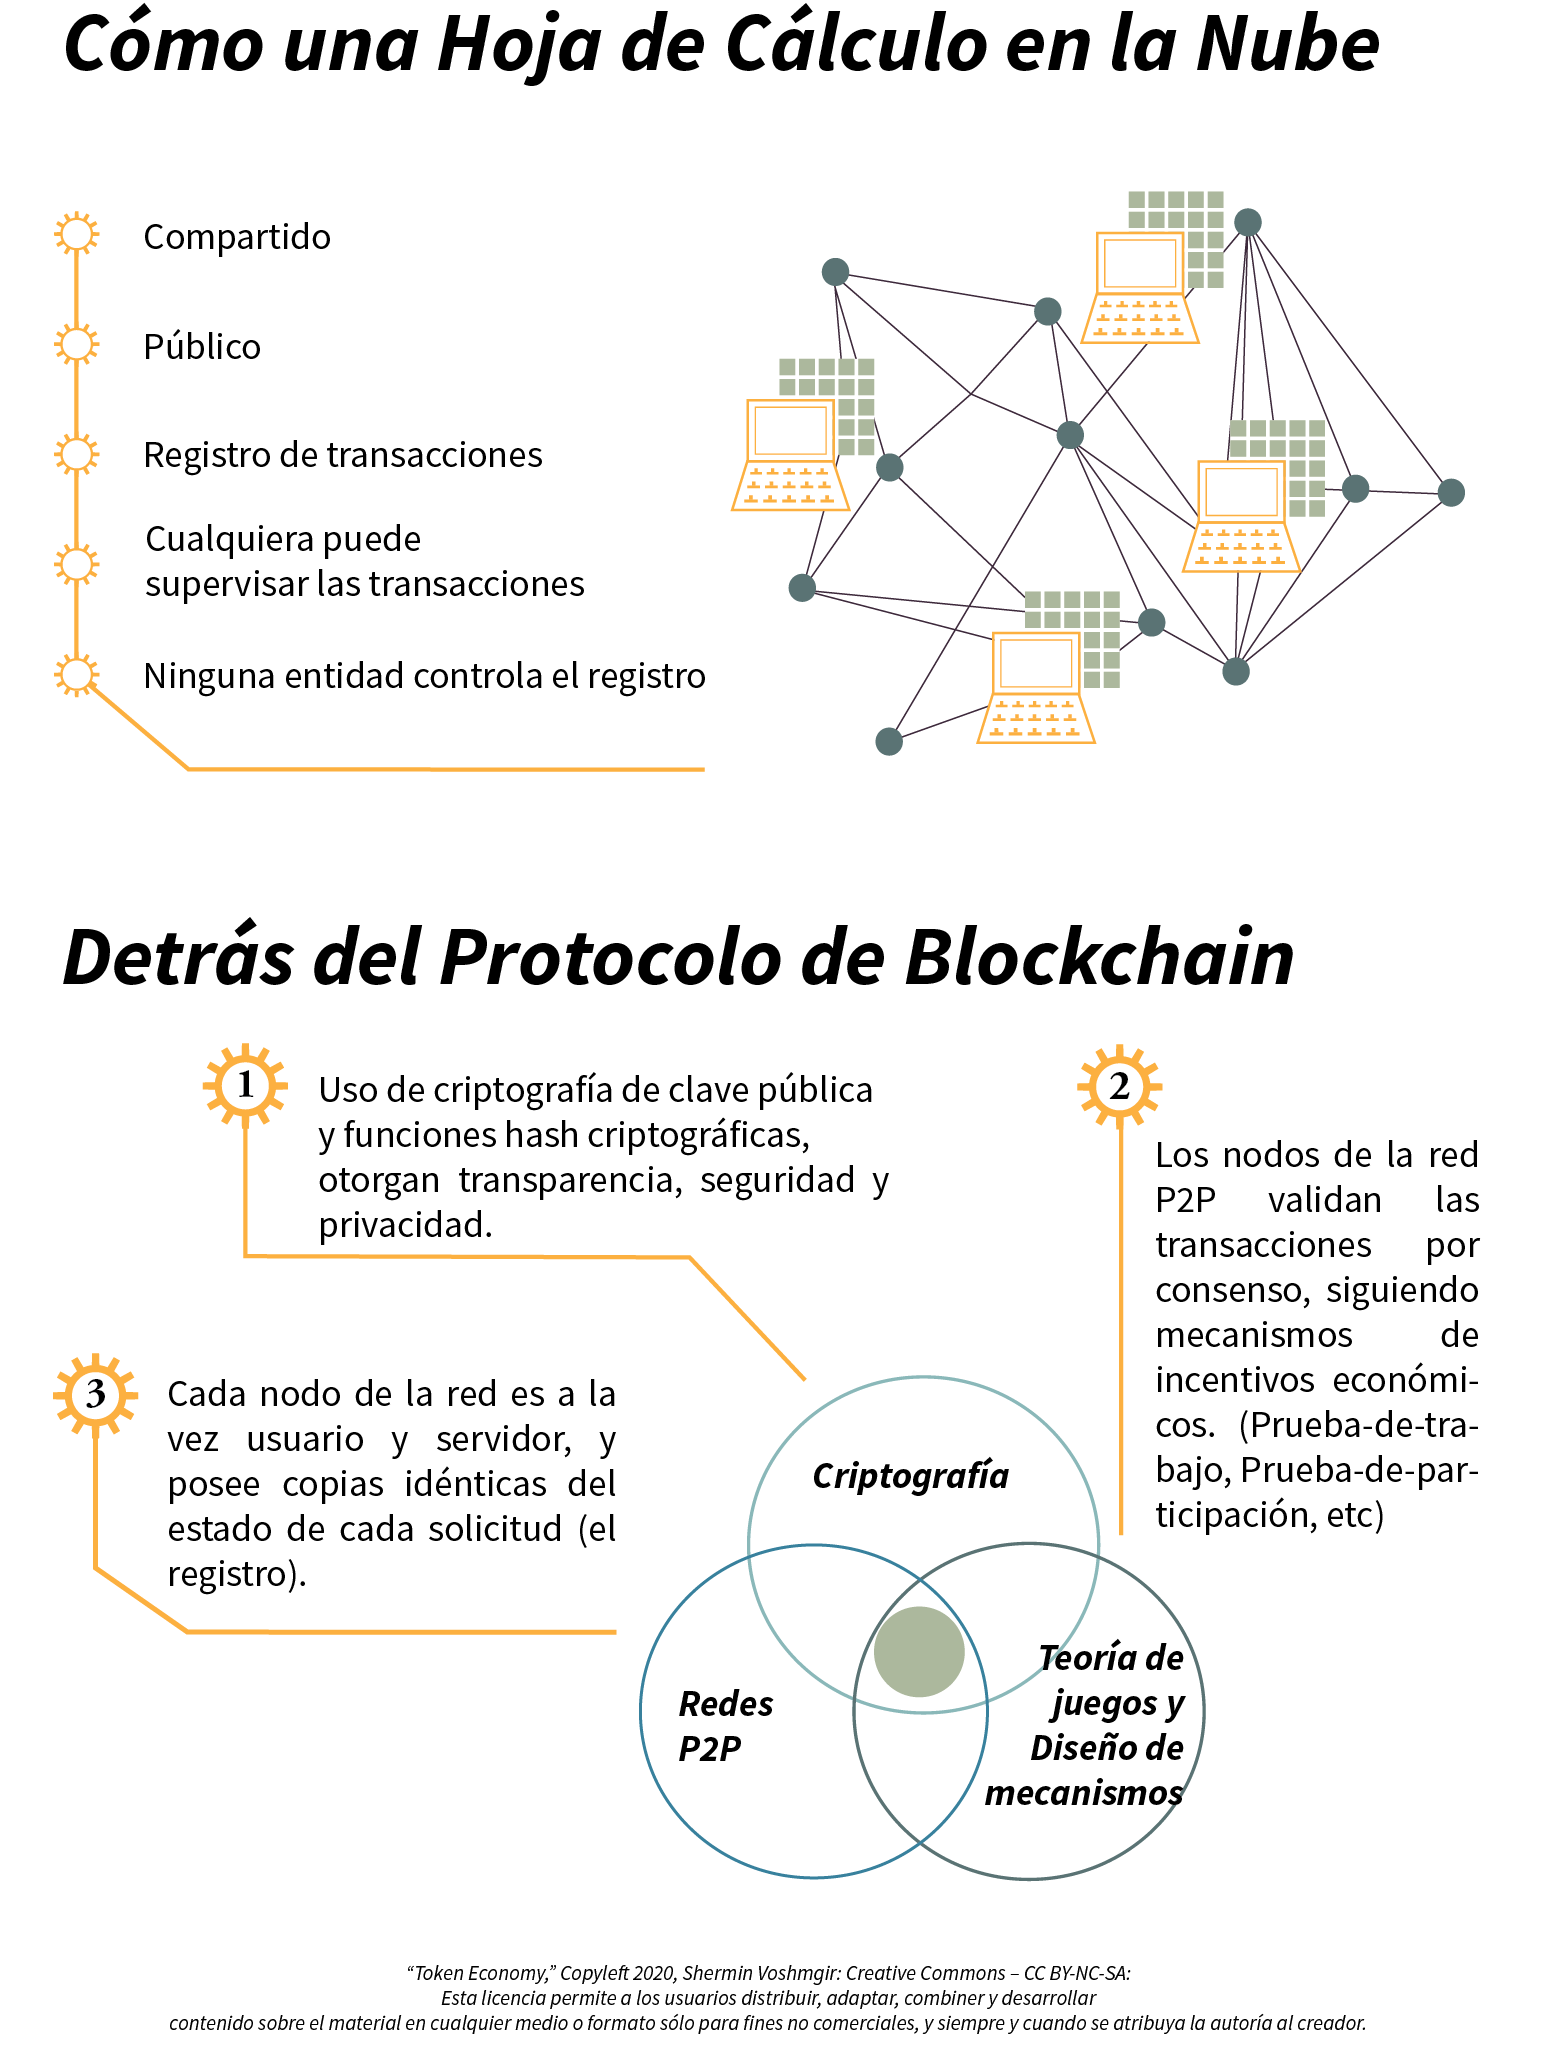
\includegraphics[width=0.8\textwidth]{Figures/venn-blockchain.png}
    \caption{Intersección de tecnologías y conceptos que componen la tecnología blockchain}
    \label{fig:blockchain-venn}
\end{figure}

En las próximas páginas se explorará en detalle la estructura y funcionamiento de la tecnología blockchain, sus características distintivas, los mecanismos de consenso que garantizan su seguridad y el papel de los contratos inteligentes como herramientas para la automatización de procesos. Además, se analizarán las ventajas y desafíos asociados a su implementación, así como su potencial de uso más allá del ámbito financiero.

\subsection{Estructura de una Blockchain}

La tecnología \textit{blockchain}, o cadena de bloques, es una estructura de datos distribuida y descentralizada donde la información se organiza en transacciones agrupadas en bloques enlazados criptográficamente. Cada bloque posee un código único, conocido como \textit{hash del bloque}, que lo identifica y sirve para enlazarlo al bloque posterior. El hash de cada bloque se genera a partir de su contenido y del hash del bloque anterior, creando así una cadena continua de bloques interconectados \cite{tripathi2023comprehensive}. En la Figura \ref{fig:blockchain-basic} se ilustra la estructura simplificada de una blockchain, donde cada bloque incluye el hash del bloque anterior, formando una cadena de bloques interconectados.

\begin{figure}[!htpb]
    \centering
    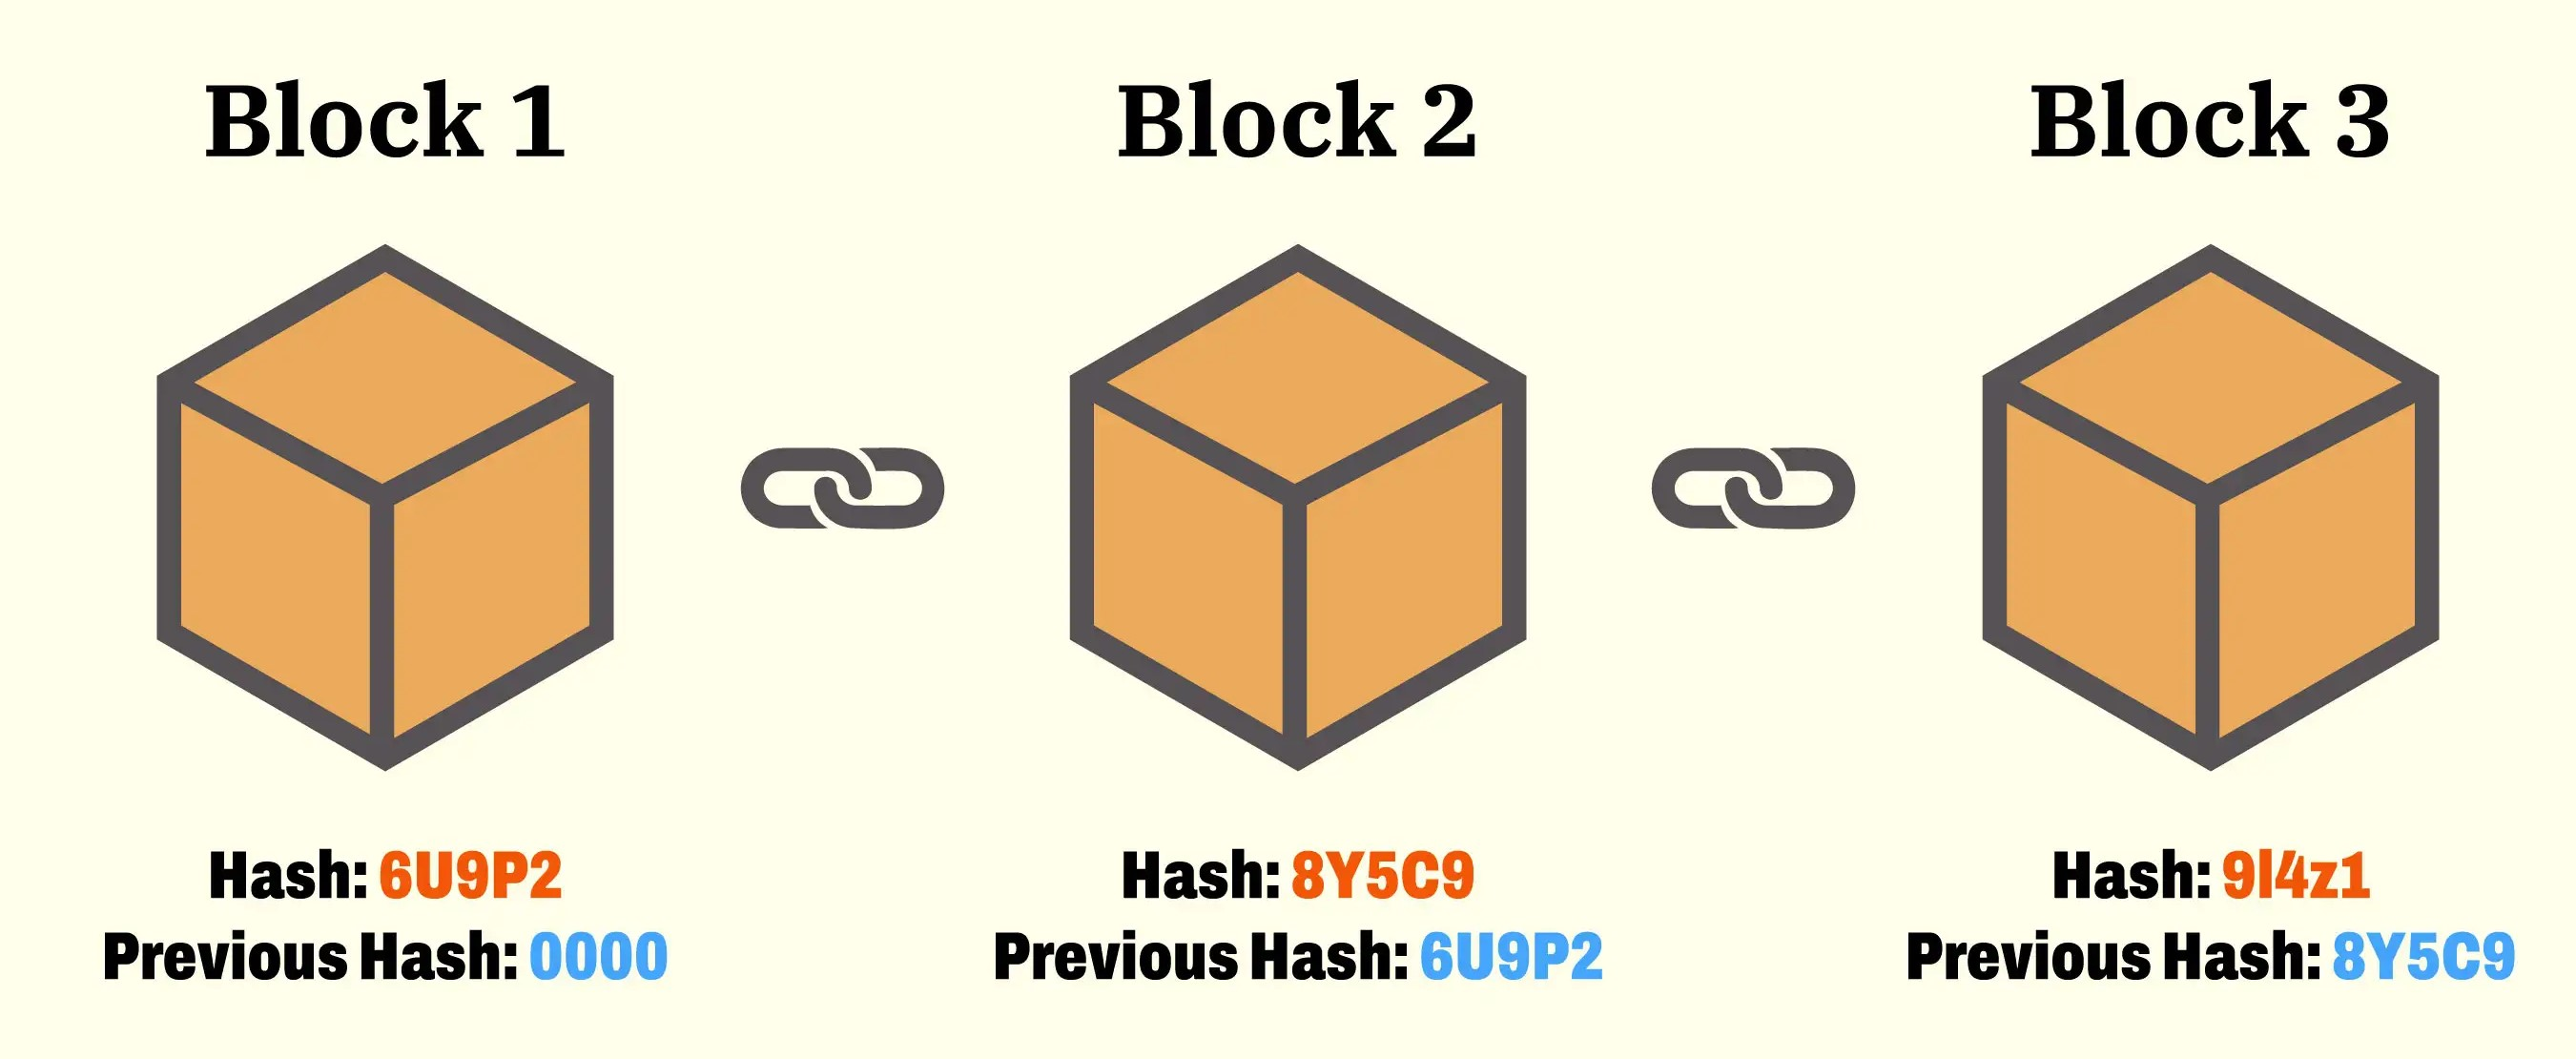
\includegraphics[width=0.8\textwidth]{Figures/blockchain-basic.jpg}
    \caption{Estructura básica de una cadena de bloques}
    \label{fig:blockchain-basic}
\end{figure}

Cada bloque de la cadena consta de un encabezado y un cuerpo \cite{tripathi2023comprehensive}. El cuerpo guarda la lista de transacciones, mientras que el encabezado contiene metadatos (que pueden variar en cada implementación). Entre los metadatos más relevantes se encuentran el código único del bloque anterior, una marca de tiempo, y el código que identifica unívocamente al bloque actual. En la Figura \ref{fig:blockchain-structure} se puede observar un esquema del contenido de un bloque de la cadena.

\begin{figure}[!htpb]
    \centering
    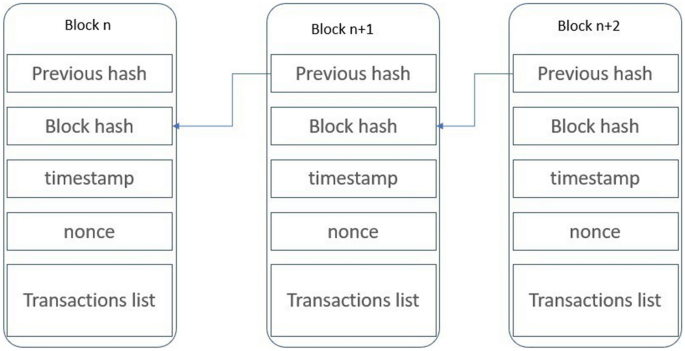
\includegraphics[width=0.8\textwidth]{Figures/blockchain-structure.png}
    \caption{Contenido de un bloque en una cadena de bloques}
    \label{fig:blockchain-structure}
\end{figure}

El hash del bloque se calcula usando funciones hash criptográficas, que son algoritmos matemáticos que transforman datos de entrada en una cadena de caracteres de longitud fija. Los códigos hash tienen la propiedad de ser rápidos de calcular, difíciles de revertir (matemáticamente imposible hacerles ingeniería inversa) y únicos para cada conjunto de datos (cualquier cambio en el contenido del bloque generará un código hash completamente diferente) \cite{pending}. Estas características permiten verificar la integridad de los datos almacenados en la cadena, ya que el código hash de un bloque se puede recalcular en cualquier momento y comparar con el código almacenado en la cadena. Si los códigos coinciden, se puede confiar en que los datos no han sido alterados; si no coinciden, se ha producido una modificación no autorizada en el contenido del bloque \cite{pending}. En la Figura \ref{fig:hash-example} se puede ver un ejemplo de los códigos generados usando un algoritmo hash a partir de dos cadenas parecidas, donde se observa que incluso un cambio mínimo en el contenido produce un hash completamente diferente. 

\begin{figure}[!htpb]
    \centering
    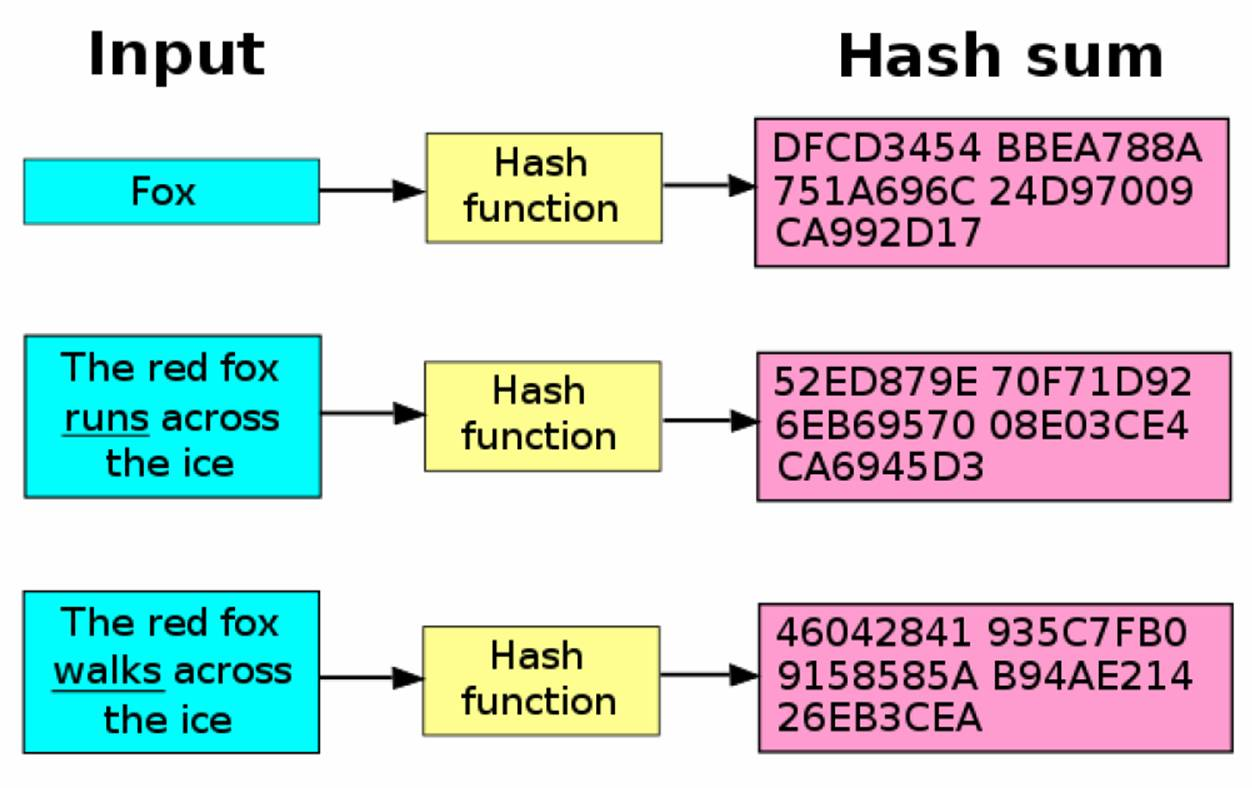
\includegraphics[width=0.8\textwidth]{Figures/hash-example.jpg}
    \caption{Ejemplo de códigos hash generados a partir de cadenas de texto}
    \label{fig:hash-example}
\end{figure}

La interconexión criptográfica entre los bloques confiere a blockchain su característica de inmutabilidad. Una vez que un bloque es añadido a la cadena, su hash se calcula a partir de su contenido y el hash del bloque anterior. Cualquier intento de alterar el contenido del bloque invalidaría este hash y, por ende, los hashes de todos los bloques subsiguientes, rompiendo la integridad criptográfica de la cadena. Este mecanismo permite la detección de cualquier intento de manipulación y la preservación de la integridad histórica del registro \cite{bulkowska2023implementation}. 

Como ya se mencionó, la blockchain es una estructura de datos distribuida y descentralizada. Ser distribuida significa que la información no se encuentra almacenada en un único servidor, sino que está distribuida en una red de computadoras interconectadas (conocidas como nodos) y cada nodo de la red mantiene una copia completa y actualizada del registro (de toda la cadena de bloques). Esto asegura su transparencia y resiliencia al no depender de un servidor central \cite{bulkowska2023implementation} propenso a ataques maliciosos y puntos únicos de fallo. Por su parte, la descentralización implica la ausencia de una autoridad central, de modo que la validación y adición de nuevos bloques se rige por un \textit{mecanismo de consenso} entre todos los nodos participantes de la red. 

Los mecanismos de consenso son algoritmos o una serie de reglas que se definen en una red distribuida para que todos los nodos (que en este caso deben guardar exactamente la misma cadena de bloques) se pongan de acuerdo sobre qué información es correcta y válida. Sin un mecanismo de consenso, la red sería vulnerables a ataques por parte de nodos maliciosos que esparzan información inválida por la red con fines de beneficio propio, pudiendo perjudicar al resto de la red. Por ejemplo, en la red Bitcoin, cada transacción representa una transferencia de fondos entre cuentas; un nodo podría difundir transacciones al resto de la red registrando que cientos de usuarios le transfirieron fondos a una cuenta en específico, si el mecanismo de consenso no definiera reglas para validar el origen legítimo de cada transacción, este nodo malicioso podría robar los fondos de los demás usuarios para beneficio exclusivo de la persona que controla ese nodo.

Cada nodo de la red blockchain ejecuta un mismo programa computacional (software) que codifica las reglas del mecanismo de consenso, definiendo cómo crear transacciones y bloques válidos, transmitirlos a la red y comprobar la validez de una transacción o bloque recibido de otro nodo antes de agregarlo a su copia local de la cadena (o descartarlo si no es válido).

Para unirse a la red, un nuevo nodo descarga una copia completa de la cadena de bloques existente, lo que le confiere una visión completa del historial de transacciones y el estado actual de la cadena \cite{bulkowska2023implementation}. Posteriormente, el nodo comienza a ejecuta el software del mecanismo de consenso. A partir de entonces, el nodo puede generar nuevas transacciones y transmitirlas a la red para ser recibidas por los demás nodos. A su vez, el nodo recibe transacciones de otros nodos y las valida mediante el mecanismo de consenso antes de añadirlas a un bloque en su copia local de la cadena \cite{bulkowska2023implementation}.

Al combinar el encadenamiento criptográfico de bloques con una red descentralizada y coordinarlo a través del mecanismo de consenso, la blockchain garantiza la integridad e inmutabilidad de la información, ya que cualquier alteración maliciosa en un bloque de la cadena modificaría su hash y rompería la consistencia posterior de la cadena, forzando a cada nodo de la red descentralizada a rechazar el bloque modificado o forzando a cada nodo a modificar los hashes de todos los bloques posteriores para recuperar la consistencia \cite{sunny2022systematic}.

En la actualidad, existen múltiples y variados algoritmos de consenso que definen distintas formas de generar un bloque válido (desde un nodo) y comprobar la validez del bloque (recibido desde otro nodo). Cada mecanismo de consenso utiliza distintas técnicas de teoría de juegos e incentivos con el objetivo de incentivar a que se unan nuevos nodos a la red (obteniendo ganancias) y desincentivar que un nodo actúe de manera maliciosa buscando un beneficio individual. Esta combinación se logra mediante esquemas donde la penalización o pérdida generada por un comportamiento malicioso supere con creces las ganancias que se puedan obtener comportándose de forma maliciosa.

El mecanismo de Prueba de Trabajo (\textit{PoW}, por sus siglas en inglés) es uno de los algoritmos de consenso más conocidos y el primero introducido en las redes blockchain por su impleementación en Bitcoin \cite{satoshi2008bitcoin}. En PoW, todos los nodos (conocidos como "mineros" en este contexto) compiten para resolver un problema matemático complejo que requiere una gran capacidad computacional. El primer nodo que logra resolver este problema matemático valida la transacción y crea el nuevo bloque incluyendo la solución en su encabezado. El resto de nodos recibe el bloque y comprueba que el problema haya sido resuelto correctamente. El nodo que resuelve el reto recibe una compensación en Bitcoin como incentivo por el aportar un bloque válido a la red. La desventaja de este algoritmo de consenso es que implica un alto costo energético debido a la carga computacional requerida para resolver el problema.

Otro mecanismo amplimente utilizando es Prueba de Participación (\textit{PoS}, por sus siglas en inglés), a diferencia de Pow, este 

 Soluciones Automatizadas para Reciclaje
Ciberataques en Argentina 2023
Marco teórico para tesis: Trazabilidad blockchain y economía circular
Alternativas a Interaction Design Foundation para programación
Políticas para la economía circular
Implementación de "Sign in with Facebook"
Tesis de Ciencias de la Computación: Resumen
Resumen de Ethereum
Conversación con Gemini

Describe y explica los mecanismos de consenso PoS y PoA. Un párrafo

por cada uno. Explica como cada uno 1. genera un bloque válido y 2. verifica que un bloque es válido. Ventajas/Desventajas de cada uno si las hay.


Mira, te dejo un ejemplo del texto donde irán para que mantengas el estilo de escritura y estructura:


```

En la actualidad, existen múltiples y variados algoritmos de consenso que definen distintas formas de generar un bloque válido (desde un nodo) y comprobar la validez del bloque (recibido desde otro nodo). Cada mecanismo de consenso utiliza distintas técnicas de teoría de juegos e incentivos con el objetivo de incentivar a que se unan nuevos nodos a la red (obteniendo ganancias) y desincentivar que un nodo actúe de manera maliciosa buscando un beneficio individual. Esta combinación se logra mediante esquemas donde la penalización o pérdida generada por un comportamiento malicioso supere con creces las ganancias que se puedan obtener comportándose de forma maliciosa.


El mecanismo de Prueba de Trabajo (\textit{PoW}, por sus siglas en inglés) es uno de los algoritmos de consenso más conocidos y el primero introducido en las redes blockchain por su impleementación en Bitcoin \cite{satoshi2008bitcoin}. En PoW, todos los nodos (conocidos como "mineros" en este contexto) compiten para resolver un problema matemático complejo que requiere una gran capacidad computacional. El primer nodo que logra resolver este problema matemático valida la transacción y crea el nuevo bloque incluyendo la solución en su encabezado. El resto de nodos recibe el bloque y comprueba que el problema haya sido resuelto correctamente. El nodo que resuelve el reto recibe una compensación en Bitcoin como incentivo por el aportar un bloque válido a la red. La desventaja de este algoritmo de consenso es que implica un alto costo energético debido a la carga computacional requerida para resolver el problema.


Otro mecanismo amplimente utilizando es Prueba de Participación (\textit{PoS}, por sus siglas en inglés), a diferencia de Pow, este ...

```

En la actualidad, existen múltiples y variados algoritmos de consenso que definen distintas formas de generar un bloque válido (desde un nodo) y comprobar la validez del bloque (recibido desde otro nodo). Cada mecanismo de consenso utiliza distintas técnicas de teoría de juegos e incentivos con el objetivo de incentivar a que se unan nuevos nodos a la red (obteniendo ganancias) y desincentivar que un nodo actúe de manera maliciosa buscando un beneficio individual. Esta combinación se logra mediante esquemas donde la penalización o pérdida generada por un comportamiento malicioso supere con creces las ganancias que se puedan obtener comportándose de forma maliciosa.

El mecanismo de Prueba de Trabajo (\textit{PoW}, por sus siglas en inglés) es uno de los algoritmos de consenso más conocidos y el primero introducido en las redes blockchain por su implementación en Bitcoin. En PoW, todos los nodos (conocidos como "mineros" en este contexto) compiten para resolver un problema matemático complejo que requiere una gran capacidad computacional. El primer nodo que logra resolver este problema matemático valida la transacción y crea el nuevo bloque incluyendo la solución en su encabezado. El resto de nodos recibe el bloque y comprueba que el problema haya sido resuelto correctamente. El nodo que resuelve el reto recibe una compensación en Bitcoin como incentivo por el aportar un bloque válido a la red. La desventaja de este algoritmo de consenso es que implica un alto costo energético debido a la carga computacional requerida para resolver el problema.

Otro mecanismo ampliamente utilizado es Prueba de Participación (\textit{PoS}, por sus siglas en inglés), a diferencia de PoW, no requiere de una alta capacidad computacional para la creación de bloques. En PoS, los nodos (conocidos como validadores) "apuestan" una cantidad de la criptomonedas como garantía de su buen comportamiento. Para generar un bloque válido, el protocolo selecciona pseudo-aleatoriamente un validador para generar el siguiente bloque, con una probabilidad de selección proporcional a la cantidad de criptomonedas que ha apostado. Una vez que el validador seleccionado crea un bloque y lo transmite a la red, los demás nodos validadores de la red simplemente comprueban que el bloque cumpla con las reglas de negocio del protocolo. Si un validador actúa de forma maliciosa, puede perder parte o la totalidad de su participación (proceso conocido como "slashing"). La principal ventaja del PoS es su eficiencia energética significativamente mayor en comparación con PoW, ya que no se requiere una minería intensiva. Además, puede ofrecer mayor escalabilidad y tarifas de transacción más bajas. Ethereum es un ejemplo de protocolo blockchain que fue implementado originalmente con PoW, pero que se actualizó para utilizar PoS debido a estas ventajas. Sin embargo, una desventaja potencial es el riesgo de centralización si la mayoría de la participación se acumula en pocos nodos, lo que podría darles un control desproporcionado sobre la red.

La Prueba de Autoridad (\textit{PoA}, por sus siglas en inglés) es otro mecanismo de consenso donde la validación de bloques se basa en la identidad y reputación de un conjunto pre-aprobado de validadores. Para generar un bloque válido, el protocolo elige una autoridad designada (del conjunto de validadores aprobados y de confianza) que tiene el derecho exclusivo de crear y firmar el nuevo bloque. Para verificar que un bloque es válido, los demás nodos de la red simplemente comprueban la firma digital del validador que lo propuso y que el bloque cumple con las reglas del protocolo. La principal ventaja del PoA es su alta velocidad de transacción, ya que solo un número limitado de validadores de confianza necesita llegar a un consenso. Esto lo hace ideal para redes privadas o consorcios donde la confianza entre los participantes ya existe. A su vez esta misma es su mayor desventaja, ya que la seguridad y el control de la red dependen de un pequeño grupo de entidades conocidas, lo que va en contra del principio de descentralización de muchas blockchains públicas.

Cada uno de los mecanismos mencionados ofrece distintos niveles de eficiencia de procesamiento, seguridad y descentralización. Durante la validación del bloque, se verifican múltiples aspectos en común en cualquiera de estos mecanismos: la correcta correspondencia del hash del bloque anterior con el almacenado en el encabezado del nuevo bloque, la validez de las transacciones de acuerdo a la lógica de negocios propia del protocolo blockchain, y que el hash del bloque propuesto haya sido generado correctamente a partir de la totalidad de su contenido.

Todo algoritmo de consenso debe asegurar que el costo de modificar un bloque de forma fraudulenta supere significativamente el beneficio potencial derivado de dicha acción \cite{satoshi2008bitcoin}. Esta característica garantiza que la red se mantenga segura y resistente a ataques \cite{buterin2013ethereum}. En el caso de Bitcoin, por ejemplo, el algoritmo de consenso Proof of Work (PoW) exige que los nodos realicen cálculos computacionales intensivos para generar nuevos bloques válidos. Aunque la validación de un bloque es de complejidad constante, la alteración de un bloque ya existente implicaría la necesidad de recalcular no solo dicho bloque, sino también todos los bloques subsiguientes. Esto convierte la modificación en un proceso extremadamente costoso en términos de recursos computacionales y energía, lo cual, sumado al rechazo de la red hacia cualquier cadena alterada, desincentiva eficazmente los intentos de manipulación \cite{satoshi2008bitcoin}.

La combinación de la red distribuida, con la estructura encadenada criptográficamente y el mecanismo de consenso, convierten a la blockchain en una base de datos que permite registrar transacciones de forma segura, transparente e inmutable, prescindiendo de una autoridad central para la administración o validación de los intercambios. En la Figura \ref{fig:blockchain-working} se presenta un esquema ilustrativo con los pasos del proceso de incorporación de una nueva transacción y su respectivo bloque en una blockchain. 

\begin{figure}[!htpb]
    \centering
    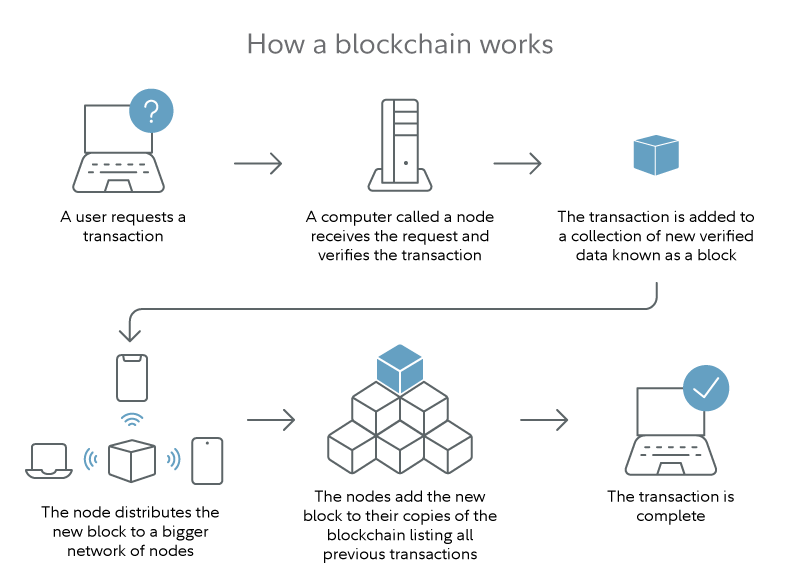
\includegraphics[width=0.8\textwidth]{Figures/block-creation.png}
    \caption{Creación de una transacción y un bloque en una blockchain}
    \label{fig:blockchain-working}
\end{figure}

El proceso de incorporación de una nueva transacción y su respectivo bloque en una blockchain se desarrolla a través de los siguientes pasos:

\begin{enumerate}
    \item Un nodo de la red crea y firma una nueva transacción con su clave privada (la firma criptográfica garantiza la autenticidad de la transacción)
    \item La transacción se propaga a través de la red distribuida, donde es recibida por cada nodo participante.
    \item Cada nodo valida la transacción individualmente, verificando la firma del remitente y asegurándose de que la transacción cumple con la lógica de negocios propia del protocolo blockchain (por ejemplo, en Bitcoin, que el remitente cuente con los fondos a tranferir). Una vez validada, la transacción se añade a un \textit{pool} de transacciones pendientes. En caso de ser inválida, simplemente se ignora y se descarta. 
    \item Cuando un nodo tiene suficiente cantidad de transacciones en su \textit{pool}, procede a seleccionar un conjunto de transacciones pendientes del \textit{pool} para formar un nuevo bloque. Este bloque incluye las transacciones seleccionadas, el hash del bloque anterior y otros metadatos (como la marca de tiempo y un \textit{nonce} para PoW). Luego, el nodo calcula el hash de este nuevo bloque y, según el algoritmo de consenso, realiza el trabajo necesario para garantizar que sea válido. En el caso de PoW, esto implica resolver un problema criptográfico que requiere una cantidad significativa de potencia computacional. En PoS, el nodo debe demostrar que posee una cantidad suficiente de fondos para participar en la validación del bloque.
    \item Una vez que el nodo ha validado el nuevo bloque (o "minado" en PoW), lo difunde a la red. Los demás nodos reciben este bloque y verifican su validez (incluyendo el hash, las transacciones y la prueba de trabajo/participación). Si el bloque es válido, cada nodo lo añade a su copia local de la cadena de bloques y descarta de su \textit{pool} de pendientes las transacciones incluidas en el bloque. Si el bloque es inválido, es rechazado por cada nodo y no se añade a la cadena.
\end{enumerate}

De esta forma, la cadena de bloques se actualiza de manera continua y descentralizada, asegurando que todos los nodos de la red mantengan una copia idéntica y consistente del registro de transacciones. Si bien en su concepción inicial las transacciones en un bloque se asociaban comúnmente a movimientos financieros \cite{satoshi2008bitcoin}, la flexibilidad inherente de la tecnología blockchain permite que los bloques contengan cualquier tipo de información estructurada \cite{bartolomeo2020introduccion}. Esta versatilidad ha sido el motor para el desarrollo de aplicaciones más complejas, destacando entre ellas los contratos inteligentes \cite{sunny2022systematic}.

\subsection{Contratos Inteligentes}

Los \textit{smart contracts}, o contratos inteligentes, son programas inmutables almacenados en una blockchain que se ejecutan automáticamente al cumplirse condiciones preestablecidas en su código \cite{bulkowska2023implementation}. Su función principal es automatizar procesos en entornos descentralizados, lo que reduce significativamente la dependencia de intermediarios humanos \cite{verma2023overview} y mejora la eficiencia operativa en múltiples sectores \cite{sunny2022systematic}.

Un contrato inteligente se concibe como un conjunto de reglas y lógica de negocio codificadas. Cada contrato posee un código (las reglas) y un estado (la información dinámica) \cite{buterin2013ethereum}. El código es inmutable una vez desplegado en la blockchain mediante una transacción, garantizando la permanencia de las reglas establecidas. Su estado, sin embargo, puede evolucionar a medida que se interactúa con el contrato a través de transacciones. Es importante destacar que, si bien se describen como "auto-ejecutables" por su automatismo al cumplir condiciones, su ejecución es llevada a cabo por los nodos de la red que validan las transacciones e integran los cambios de estado en la cadena \cite{buterin2013ethereum}. Tanto el código como el estado del contrato se almacenan en la blockchain, asegurando su transparencia y disponibilidad pública. Por ejemplo, un contrato inteligente podría gestionar un sistema de votación, donde los participantes envían sus votos y el contrato contabiliza automáticamente los resultados al finalizar el periodo de votación. En la Figura \ref{fig:smart-contract-process} se ilustra el proceso de creación y ejecución de un contrato inteligente, describiendo las etapas desde su definición hasta su implementación y ejecución en la blockchain.

% TODO: use the votation example in this figure to explain the flow of contract creation and execution.
\begin{figure}[!htpb]
    \centering
    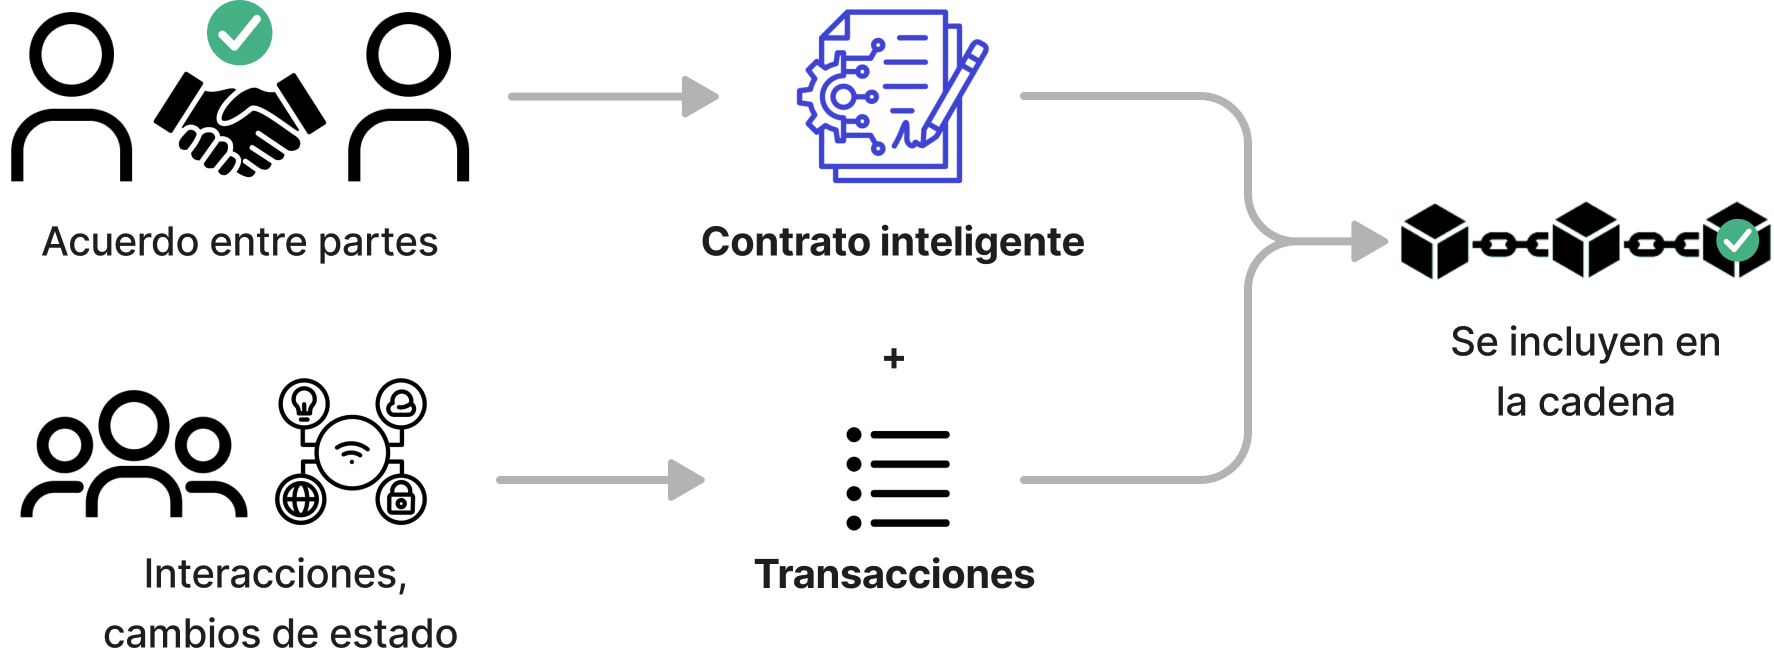
\includegraphics[width=0.8\textwidth]{Figures/smart-contract-process.png}
    \caption{Proceso de creación y ejecución de un contrato inteligente}
    \label{fig:smart-contract-process}
\end{figure}

Para el desarrollo y ejecución de contratos inteligentes, se emplean lenguajes de programación específicos adaptados a cada plataforma blockchain \cite{bartolomeo2020introduccion}. Un ejemplo prominente es \textit{Solidity} \cite{taherdoost2023smart}, utilizado en Ethereum, un lenguaje orientado a objetos diseñado para esta finalidad. Estos contratos pueden interactuar entre sí y con el estado global de la blockchain, habilitando la creación de aplicaciones descentralizadas (conocidas también como \textit{dApps}, por sus siglas en inglés) que operan de forma autónoma y sin intermediarios en la red \cite{buterin2013ethereum}.

Sin embargo, los contratos inteligentes enfrentan limitaciones inherentes a las infraestructuras blockchain, principalmente en términos de escalabilidad \cite{kalajdjieski2023databases}. A diferencia de los sistemas centralizados que permiten ejecución paralela y optimización con bases de datos indexadas, los smart contracts operan bajo modelos de ejecución secuencial y replicación completa en cada nodo \cite{taherdoost2023smart}. Esto impacta directamente su rendimiento y complejiza la implementación de algoritmos avanzados. Desde la perspectiva de la ingeniería de software, el desarrollo de contratos inteligentes introduce restricciones no triviales: el código inmutable, los costos asociados al almacenamiento en cadena, la ausencia de llamadas externas directas y los modelos de estado global distribuido. Estas particularidades exigen la adopción de nuevas metodologías y prácticas de diseño seguro, control de flujos y validación estática, muchas de las cuales aún se encuentran en proceso de estandarización \cite{taherdoost2023smart, cepal2021economia}.

En síntesis, los contratos inteligentes constituyen una herramienta computacional que expande las fronteras de la programación distribuida y descentralizada. Si bien su potencial transformador es innegable \cite{taherdoost2023smart}, su desarrollo robusto y seguro representa un desafío activo que abarca múltiples dominios de la computación: desde la teoría de lenguajes formales \cite{hoskinson2017we} y la arquitectura de sistemas distribuidos, hasta la verificación de software, la criptografía aplicada y la integración de datos externos confiables \cite{taherdoost2023smart}.

Debido a la aparición los contratos inteligentes, la tecnología blockchain ha trascendido su origen ligado a las criptomonedas para convertirse en un paradigma disruptivo con aplicaciones transversales en múltiples dominios \cite{bartolomeo2020introduccion, vaigandla2023review}. Se posicionan como un componente fundamental y un impulsor clave de gran parte de las nuevas y complejas soluciones basadas en blockchain, especialmente aquellas que buscan automatizar procesos y gestionar la lógica de negocio directamente en la cadena \cite{sharabati2024blockchain}. Si bien los contratos inteligentes representan una tecnología prometedora, aún se encuentran en una etapa incipiente, lo que implica la existencia de numerosos aspectos por perfeccionar \cite{taherdoost2023smart}. En un contexto más amplio, la tecnología blockchain, incluyendo a los contratos inteligentes, ofrece una serie de ventajas fundamentales y limitaciones inherentes que la distinguen de los sistemas de almacenamiento de datos tradicionales.

\subsection{Desafíos y Oportunidades}

Las características inherentes de la blockchain, detalladas previamente, se traducen en una serie de ventajas que la distinguen de tecnologías tradicionales. La descentralización propia de su diseño y la consecuente eliminación de intermediarios resultan en una mayor confianza \cite{rejeb2023role} y eficiencia operativa al prescindir de autoridades centrales \cite{sharabati2024blockchain}. La arquitectura basada en registros inmutables garantiza transparencia y trazabilidad completa \cite{sharabati2024blockchain}, permitiendo un historial verificable de cualquier activo o evento, lo cual es crucial para casos de uso como certificación \cite{bartolomeo2020introduccion}, logística \cite{bartolomeo2020introduccion, rejeb2023role} y gestión de residuos \cite{bulkowska2023implementation}. La inmutabilidad de los datos, reforzada por la seguridad criptográfica, asegura la integridad de la información \cite{sunny2022systematic} y una resistencia robusta a manipulaciones maliciosas y puntos únicos de falla \cite{bartolomeo2020introduccion}. Además, la capacidad de automatización de aplicaciones mediante contratos inteligentes optimiza la eficiencia y confiabilidad operativa al ejecutar condiciones lógicas de forma autónoma \cite{bartolomeo2020introduccion}. En conjunto, estas propiedades confieren a blockchain una aplicabilidad transversal que la consolida como una tecnología habilitadora para la transformación digital en sectores diversos como finanzas, salud, IoT, energía, educación y ciudades inteligentes.

Sin embargo, a pesar de sus beneficios, la tecnología blockchain también enfrenta desafíos y limitaciones significativos. Uno de los principales desafíos es la escalabilidad y el rendimiento \cite{tripathi2023comprehensive}. Las blockchains actuales suelen presentar un bajo \textit{throughput} en comparación con los sistemas centralizados \cite{baralla2023waste}, lo cual restringe su aplicación en escenarios de alta frecuencia transaccional. Esto se debe inherentemente a la necesidad de alcanzar un consenso distribuido y a la replicación completa de datos en todos los nodos \cite{tripathi2023comprehensive}. Otro reto importante es la interoperabilidad limitada, que dificulta la integración fluida entre distintas plataformas blockchain con infraestructuras externas preexistentes \cite{tripathi2023comprehensive}. En entornos públicos, la privacidad es una preocupación, ya que, aunque los usuarios pueden operar de forma seudónima, la visibilidad total de las transacciones en la cadena puede comprometer datos sensibles \cite{diez2023web, rennock2018blockchain}. Además, existen vulnerabilidades técnicas inherentes, como el ataque del 51\%, el doble gasto, los ataques Sybil, y la posibilidad de errores en contratos inteligentes mal programados, que requieren atención constante \cite{diez2023web}. La irreversibilidad de las transacciones, si bien es una garantía de seguridad, puede ser problemática ante vulnerabilidades de programación, errores o fraudes, ya que las operaciones registradas no pueden deshacerse \cite{taherdoost2023smart}. Por último, las limitaciones de almacenamiento representan un desafío práctico, dado que los nodos deben almacenar volúmenes crecientes de información, lo cual no escala eficientemente en redes de gran tamaño \cite{taherdoost2023smart}.

Estos desafíos, aunque significativos, están siendo abordados activamente por la investigación y el desarrollo en la comunidad blockchain. La constante evolución de la tecnología y la aparición de nuevas soluciones buscan mitigar estas limitaciones, abriendo el camino para una adopción más amplia \cite{tripathi2023comprehensive, baralla2023waste, taherdoost2023smart}. En este contexto de evolución y superación de barreras, la blockchain ha demostrado su potencial para transformar diversos sectores y abarcar numerosos casos de uso.

% \subsection{Casos de Uso}

En el sector financiero, blockchain ha generado disrupción mediante soluciones para pagos directos (con las llamadas criptomonedas), emisión de bonos, transferencias internacionales y operaciones en mercados de capital \cite{bartolomeo2020introduccion}. Instituciones como Santander y la Bolsa de Comercio de Santiago han adoptado esta tecnología para simplificar transacciones, automatizar registros y eliminar intermediarios \cite{bartolomeo2020introduccion}. Gracias a su estructura descentralizada y sus mecanismos criptográficos, blockchain permite mejorar la trazabilidad de los activos financieros. Pero si bien su uso en finanzas ha sido el más destacado, la tecnología blockchain ha demostrado ser versátil y aplicable a una amplia gama de sectores, cada uno con sus propias necesidades y desafíos.

A nivel gubernamental, blockchain ofrece nuevas herramientas para la modernización del Estado. Permite la gestión segura y verificable de identidades digitales, la trazabilidad de procesos administrativos, y la implementación de sistemas de votación transparentes \cite{vaigandla2023review}. Iniciativas como la European Blockchain Partnership buscan establecer una infraestructura digital pública para servicios intergubernamentales \cite{diez2023web}. Proyectos como QualiChain exploran aplicaciones en el sector público, como la verificación de credenciales profesionales y la gestión automatizada de elegibilidad en concursos públicos \cite{diez2023web}.

Para el sector de la salud, blockchain permite almacenar registros médicos de manera segura y distribuida, mejorando la interoperabilidad entre instituciones, garantizando la integridad de los datos y permitiendo un mayor control por parte de los pacientes \cite{sunny2022systematic, }. También es utilizado en la trazabilidad de la cadena de suministro farmacéutica y en la supervisión de ensayos clínicos, donde se requiere un alto nivel de confianza y garantizar cumplimiento normativo \cite{vaigandla2023review}.

Aplicaciones de blockchain en el rubro de la educación incluyen la emisión y verificación de certificados académicos inmutables y descentralizados. Universidades como Nicosia o la de Murcia ya utilizan blockchain para certificar diplomas y logros \cite{diez2023web}. Iniciativas como Blockcerts o el pasaporte educativo propuesto por la Unión Europea buscan facilitar la movilidad académica y reducir la falsificación documental. También se exploran aplicaciones como exámenes autoevaluables con contratos inteligentes, recompensas por desempeño y la gestión segura de registros estudiantiles \cite{diez2023web}.

También se está utilizando tecnología blockchain para crear mercados descentralizados para el comercio de energía entre pares. En este caso, su uso mejora la gestión de certificados de energías renovables, y optimiza la trazabilidad de producción y consumo energético \cite{sunny2022systematic, vaigandla2023review}.

En el ámbito de la gestión de la cadena de suministro (SCM), blockchain proporciona una plataforma confiable para garantizar la trazabilidad, autenticidad y visibilidad en tiempo real de productos y materiales \cite{torres2022tendencias, sharabati2024blockchain}. Empresas como IBM, Maersk y FedEx han implementado soluciones blockchain para monitorear inventarios, registrar pagos y reducir disputas logísticas \cite{tripathi2023comprehensive}. Casos como el de Dervinsa en Argentina, que certifica la calidad de productos derivados de residuos de vinificación, y otras iniciativas que aplican trazabilidad a alimentos y textiles, muestran cómo esta tecnología fortalece el control de calidad y la confianza en los mercados \cite{bartolomeo2020introduccion}. Además, en contextos más amplios, blockchain permite una sincronización eficiente entre departamentos, la reducción de riesgos de falsificación y la mejora general de la sostenibilidad operativa \cite{sunny2022systematic}.

Dentro de modelos de economía circular, blockchain se posiciona como un facilitador para monitorear ciclos de vida de productos y materiales, ofreciendo transparencia y responsabilidad en la gestión de residuos \cite{bulkowska2023implementation, baralla2023waste}. Diversos tipos de residuos, desde plásticos y vidrio hasta electrónicos y biomédicos, pueden ser gestionados de forma más eficiente mediante el uso de contratos inteligentes que automatizan verificaciones, recompensas e interacciones entre actores de la cadena \cite{baralla2023waste}. Asimismo, han surgido propuestas innovadoras como la generación de pasaportes digitales de productos y esquemas de incentivos sostenibles, promoviendo hábitos de consumo responsables y nuevos modelos de negocio circulares \cite{baralla2023waste}.

En IoT, facilita la recolección y gestión segura de datos en tiempo real \cite{sunny2022systematic}. En contabilidad y auditoría, posibilita libros contables distribuidos con transparencia total y reducción de fraudes \cite{bartolomeo2020introduccion}. También se emplea en caridad y donaciones, trazabilidad inmobiliaria y movilidad inteligente \cite{bartolomeo2020introduccion}. 

Estos variados casos de uso evidencian cómo blockchain puede transformar modelos tradicionales mediante estructuras distribuidas, reglas codificadas y registros inmutables. Su implementación efectiva puede contribuir a una mayor eficiencia, confianza y sostenibilidad en distintas áreas del desarrollo económico, social y tecnológico.

Uno de los ámbitos donde esta tecnología está adquiriendo un protagonismo creciente es en la economía circular. La necesidad de trazar el flujo de materiales, certificar la autenticidad de los procesos productivos y garantizar la gestión responsable de residuos ha posicionado a blockchain como una herramienta protagónica para habilitar modelos circulares sostenibles. En particular, su capacidad para registrar datos inmutables y automatizar interacciones mediante contratos inteligentes permite estructurar sistemas de trazabilidad que no sólo mejoran la eficiencia, sino que también fortalecen la confianza entre actores y fomentan la rendición de cuentas \cite{sharabati2024blockchain, rejeb2023role}. A continuación, se analizará con mayor profundidad el uso de blockchain para trazabilidad de materiales en la cadena de suministros y para la implementación de estrategias de economía circular.

\section{Economía circular}

La economía circular es un enfoque alternativo al modelo económico lineal tradicional, que nace con el objetivo transformar de forma sostenible la forma en que la sociedad produce, consume y gestiona los recursos naturales.

Desde la Revolución Industrial, la economía global ha operado principalmente bajo un modelo lineal de "extraer, producir y consumir", caracterizado por la explotación de recursos naturales y la generación masiva de residuos \cite{cerda2016economia}. En este modelo económico, los recursos son extraídos de la naturaleza, transformados en productos, consumidos y finalmente desechados al terminar su vida útil. Este enfoque, aunque ha impulsado un crecimiento económico mundial sin precedentes, ha generado sobreexplotación y degradación de ecosistemas. La deforestación, pérdida de biodiversidad, contaminación del agua, generación masiva de residuos y escasez de recursos no renovables son algunas de las consecuencias negativas de este enfoque extractivo a gran escala. A medida que la población mundial y la demanda de recursos continúan creciendo, la insostenibilidad de este modelo a largo plazo se hace cada vez más evidente \cite{clima2022book}.

En contraste con la economía lineal, la economía circular propone un sistema en el que los recursos se mantienen en uso durante el mayor tiempo posible, se reciclan y se reutilizan, minimizando la generación de residuos y reduciendo la extracción de materias primas \cite{ellenmacarthurfoundation2022}. La economía circular propone un cambio radical de paradigma, al concebir los sistemas productivos y de consumo como ciclos cerrados. Este enfoque se basa en los principios de diseño ecológico, la reutilización de materiales y la regeneración de los sistemas naturales, con el objetivo de crear un sistema económico más sostenible y resiliente. La diferencia estructural entre la economía lineal y la economía circular se hace evidente al ilustrar el flujo de recursos en ambos modelos, como se muestra en la Figura \ref{fig:circular-linear-economy-comparison}.

\begin{figure}[!htpb]
    \centering
    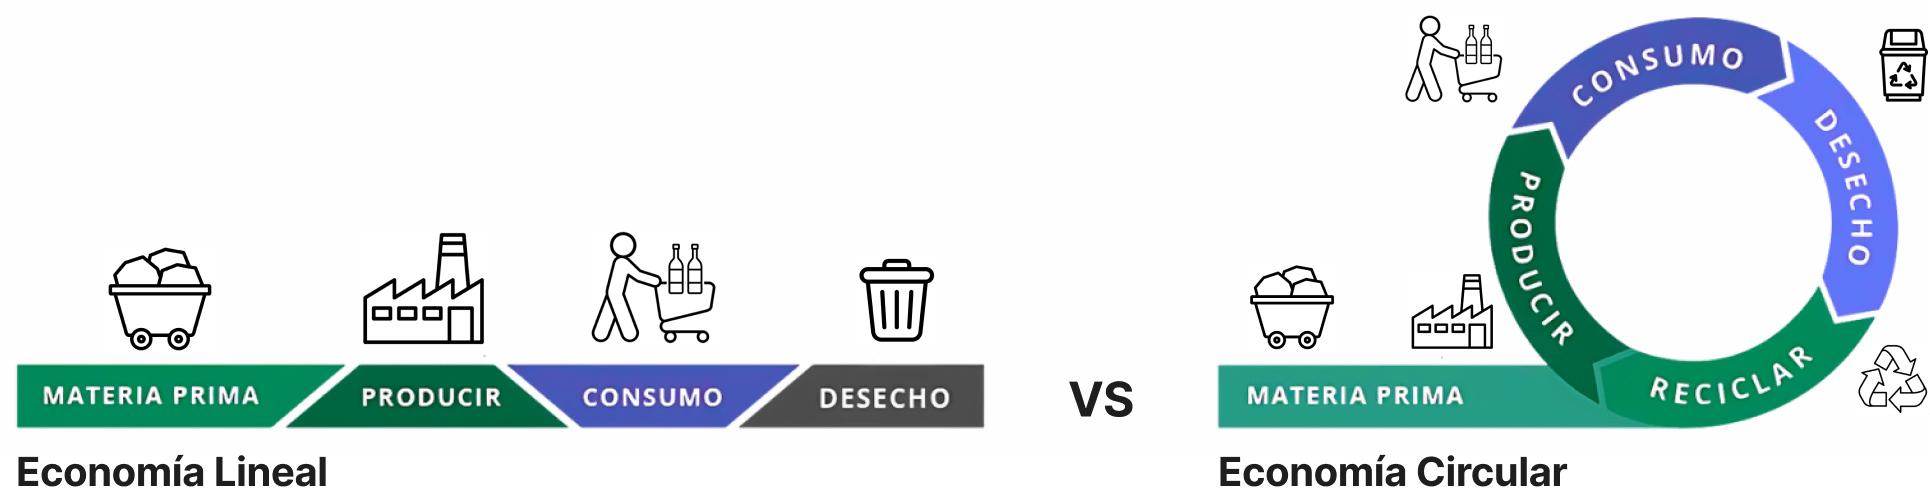
\includegraphics[width=0.8\textwidth]{Figures/circular-linear-economy-comparison.png}
    \caption{Comparación entre la economía lineal y la economía circular}
    \label{fig:circular-linear-economy-comparison}
\end{figure}

En el enfoque lineal, la cadena de suministro de materiales se organiza como un proceso unidireccional: los recursos son extraídos, transformados en productos, consumidos y finalmente desechados. Este modelo ignora el valor residual de los materiales, no contempla mecanismos para reincorporar los productos al ciclo productivo una vez finalizada su vida útil y, en consecuencia, genera una creciente acumulación de residuos. En contraste, la economía circular redefine el papel de la cadena de suministros, transformándola en una red cerrada y regenerativa. Con este enfoque, la cadena se vuelve más dinámica e interdependiente, integrando bucles de retroalimentación entre los diferentes actores de la cadena de valor, incluyendo a consumidores, productores, proveedores y gestores de residuos. 

A nivel sistémico, la economía circular se concibe como una evolución hacia un sistema más integrado, resiliente y sostenible. Su implementación es paulatina, en forma de transición desde el modelo lineal predominante hacia un modelo circular. Esta transición requiere una transformación estructural en los sistemas productivos en múltiples niveles: diseño de productos, procesos logísticos, distribución y gestión del fin de vida útil. Entre los habilitadores clave de este proceso de transición, se encuentra la trazabilidad, entendida como la capacidad de rastrear el origen, el uso y el destino de materiales y productos a lo largo de toda su vida útil. La trazabilidad permite verificar compromisos ambientales, controlar impactos, optimizar la logística inversa y empoderar tanto a consumidores como a instituciones para adoptar decisiones basadas en información confiable.

En la actualidad existen desafíos culturales, normativos y tecnológicos que dificultan la implementación de la economía circular a gran escala. La transición de los sistemas productivos requiere inversión en infraestructura, marcos regulatorios adecuados y políticas de incentivos claros. Asimismo, implica repensar la educación y la formación de trabajadores para adaptarse a nuevas dinámicas laborales. En muchos contextos, como América Latina y el Caribe, también se han identificado limitaciones institucionales y de gobierno que deben ser abordadas para permitir una adopción efectiva del modelo.

Es importante destacar que esta transición ya se encuentra en marcha. Numerosos países, regiones y sectores productivos han comenzado a incorporar principios circulares en sus estrategias de desarrollo, en muchos casos impulsados por marcos regulatorios, acuerdos internacionales y metas vinculadas a la sostenibilidad ambiental. En este contexto, las políticas públicas han asumido un rol central como motores de adopción, ofreciendo instrumentos normativos, fiscales y de gobernanza que facilitan la transformación del sistema económico. %A continuación, se analizarán algunas políticas sustentables relevantes para avanzar hacia una economía más circular y resiliente.

\subsection{Políticas sustentables}

En el proceso de transición hacia modelos de desarrollo más sostenibles, la Unión Europea ha asumido un rol pionero en la implementación de políticas públicas alineadas con la economía circular. Iniciativas como el Pacto Verde Europeo y la Ley Europea del Clima han consolidado a Europa como un referente global en materia de sustentabilidad ambiental. Estas políticas no solo promueven la descarbonización de la economía, sino que también introducen principios de circularidad en sectores como la industria, la energía, la movilidad y la gestión de residuos, reconfigurando las cadenas de suministro hacia sistemas más regenerativos, transparentes y trazables.

Sin embargo, el mayor hito internacional en la construcción de una visión compartida sobre sustentabilidad ha sido la adopción de los Objetivos de Desarrollo Sostenible (ODS) de Naciones Unidas en 2015. Este conjunto de 17 objetivos interconectados, acompañados por 169 metas y más de 230 indicadores, propone una agenda universal que orienta las políticas públicas hacia un desarrollo económico, social y ambiental equilibrado para 2030.

\begin{figure}[!htpb]
    \centering
    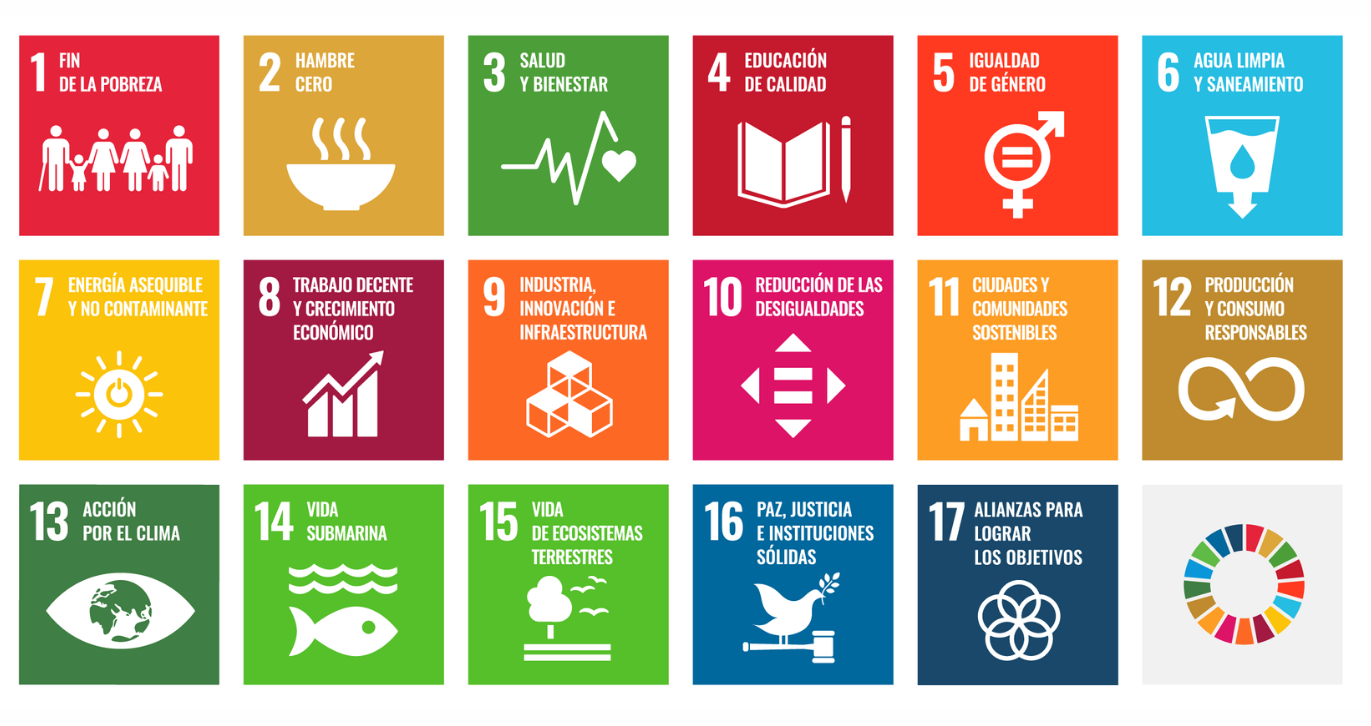
\includegraphics[width=0.8\textwidth]{Figures/ods.png}
    \caption{Objetivos de Desarrollo Sostenible (ODS) de Naciones Unidas}
    \label{fig:ods}
\end{figure}

El objetivo general de los ODS es erradicar la pobreza, proteger el planeta y garantizar la paz y prosperidad para todas las personas. En relación con la economía circular, se identifican un conjunto de objetivos particularmente relevantes que guían tanto los marcos normativos como las estrategias de innovación en producción, consumo y gestión de residuos:

\begin{itemize}
\item \textbf{ODS 7: Energía asequible y no contaminante.}\footnote{\url{https://www.un.org/sustainabledevelopment/es/energy/}} Promueve el acceso universal a fuentes de energía limpias, eficientes y modernas, fundamentales para la transición a una economía circular descarbonizada.
\item \textbf{ODS 11: Ciudades y comunidades sostenibles.}\footnote{\url{https://www.un.org/sustainabledevelopment/es/cities/}} Plantea la necesidad de gestionar de manera integrada los recursos urbanos, incluyendo residuos, infraestructura y movilidad, en articulación con una trazabilidad eficiente de los flujos materiales.
\item \textbf{ODS 12: Producción y consumo responsables.}\footnote{\url{https://www.un.org/sustainabledevelopment/es/sustainable-consumption-production/}} Es el núcleo del paradigma circular, impulsando el diseño sostenible de productos, el uso eficiente de recursos, la minimización de residuos y la promoción de modelos de cadena de suministro regenerativos.
\item \textbf{ODS 13: Acción por el clima.}\footnote{\url{https://www.un.org/sustainabledevelopment/es/climate-change-2/}} Vincula la circularidad con la reducción de emisiones y la adaptación al cambio climático, incentivando políticas que rediseñen los sistemas productivos de alto impacto ambiental.
\end{itemize}

Los ODS han generado un marco de referencia común que ha influido fuertemente en las agendas de sostenibilidad a nivel global, incluyendo América Latina. Aunque en la región la adopción de políticas circulares aún es incipiente en comparación con Europa, se observan avances significativos en la última década. Por ejemplo, varios países han comenzado a incorporar la responsabilidad extendida del productor, prohibiciones de plásticos de un solo uso y normativas orientadas a la reutilización y reciclado de materiales. Estas políticas buscan reestructurar las cadenas de valor y fomentar prácticas productivas y logísticas compatibles con los principios de circularidad.

En Argentina, la Estrategia Nacional de Consumo y Producción Sostenibles se destaca como el instrumento central para avanzar hacia la economía circular. La estrategia integra medidas normativas, educativas, tecnológicas y financieras, orientadas a fortalecer la sostenibilidad en toda la cadena de producción y consumo. Promueve activamente el uso de tecnologías limpias, la gestión sostenible de recursos, y la incorporación de criterios ambientales en compras públicas, reconociendo el rol central de la trazabilidad como mecanismo para garantizar la transparencia, eficiencia y cumplimiento normativo en los sistemas productivos y sus cadenas de suministro.

% Si bien estos esfuerzos representan un paso importante, los desafíos estructurales persisten. La región enfrenta obstáculos en términos de infraestructura, financiamiento, coordinación institucional y disponibilidad de información confiable. A pesar de ello, el impulso dado por los ODS ha generado una convergencia regional que permite imaginar una transición hacia modelos circulares, sostenida por políticas públicas que consideran no sólo las metas globales, sino también las realidades locales.

Estas políticas dejan ver que la transformación hacia una economía circular no puede pensarse sin una reconfiguración de las cadenas de suministro, que constituyen la columna vertebral de los sistemas productivos. La implementación de políticas sustentables, tanto en Europa como en América Latina, ha puesto en evidencia la necesidad de contar con mecanismos que permitan monitorear, verificar y optimizar el flujo de materiales a lo largo de todo el ciclo de vida de los productos. En la siguiente sección se abordará con mayor detalle cómo se articula esta relación entre cadenas de suministro y trazabilidad, y cuál es su rol estratégico en la transición hacia un modelo económico circular.

\subsection{Cadena de suministro}

En el contexto de la economía circular, la cadena de suministro asume una nueva lógica de funcionamiento. Pasa de ser una secuencia finita de pasos que culminan con el consumo y disposición del producto, a transformarse en un sistema cíclico, en el cual los productos son diseñados para permanecer en uso el mayor tiempo posible y ser reutilizados, reacondicionados o reciclados. 

La cadena de suministro constituye el entramado logístico, operativo y estratégico que permite el flujo de materiales, información y recursos desde la extracción de materias primas hasta la llegada de un producto al consumidor final. Este sistema complejo involucra a múltiples actores: proveedores, fabricantes, distribuidores, minoristas, consumidores y, en el caso del modelo circular, gestores de residuos y autoridades regulatorias. Su objetivo es garantizar que los bienes y servicios se produzcan y entreguen de manera eficiente, segura y rentable. 

\begin{figure}[!htpb]
    \centering
    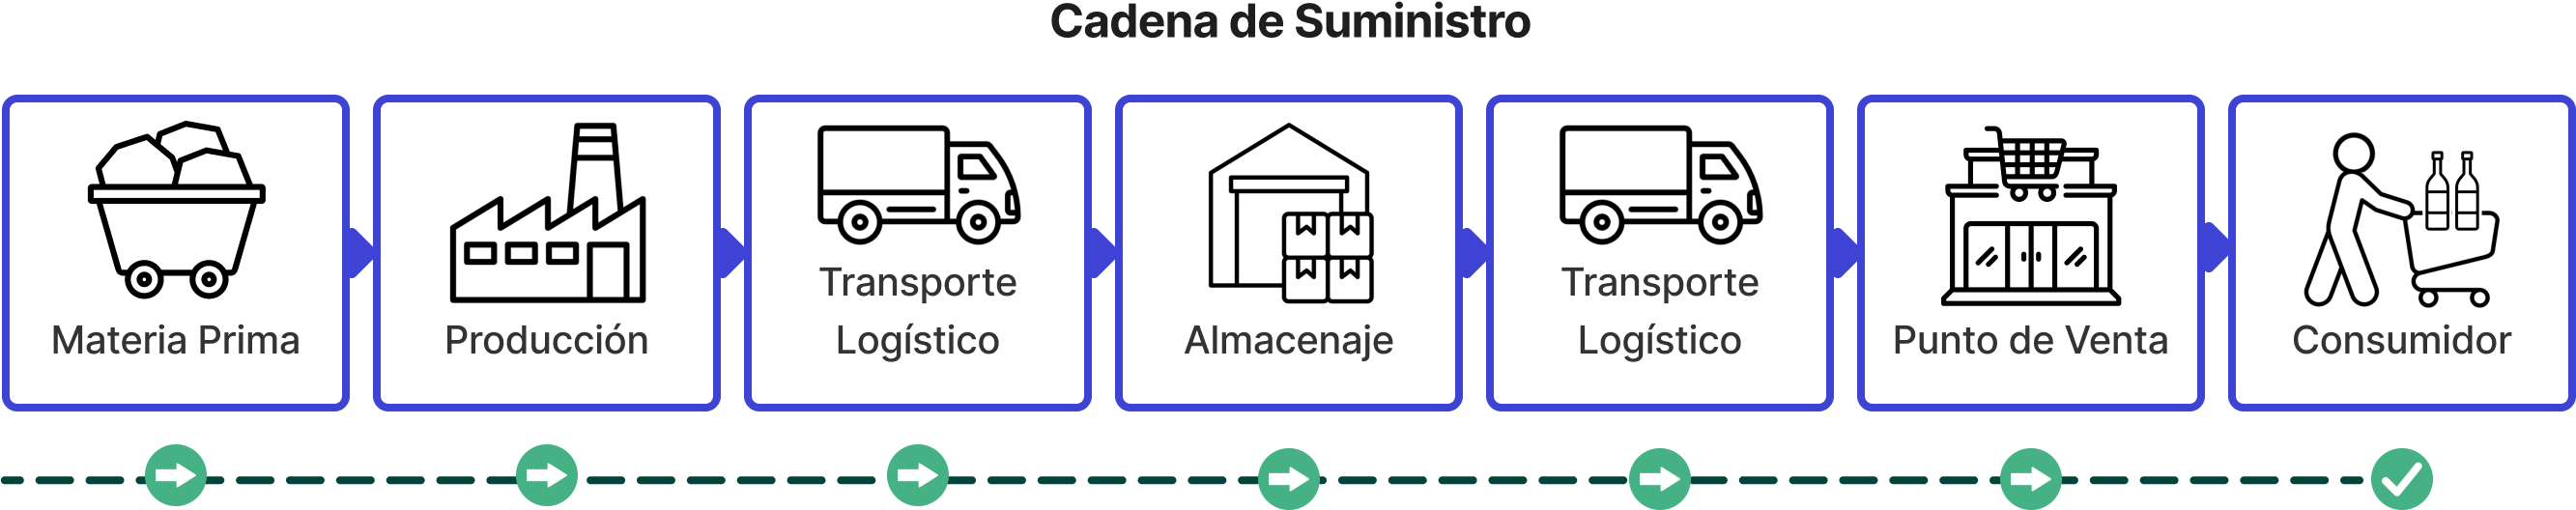
\includegraphics[width=0.8\textwidth]{Figures/supply-chain.png}
    \caption{Componentes de una cadena de suministro}
    \label{fig:supply-chain}
\end{figure}

A lo largo de los años, las cadenas de suministro se han establecido para maximizar la eficiencia y reducir costos en la producción de productos. Con este objetivo claro, es que se ha dividido el proceso en etapas y se aplican herramientas, procesos y tecnologías diversas para optimizar cada una de ellas, desde la adquisición de materias primas hasta la distribución final. Sin embargo, la maximización de la eficiencia en este modelo lineal, sin preocuparse por el destino del producto luego de su uso, ha generado efectos secundarios adversos en el medioambiente que, como ya se mencionó, han llevadoa la necesidad de un modelo sostenible en el tiempo.

Transicionar una cadena de suministros desde un modelo lineal hacia uno circular implica una inversión en rediseño de productos, procesos y creación de nuevas relaciones y colaboraciones entre los actores involucrados. En muchos casos los productores distintos actores de la cadena lo perciben como una inversión sin retorno inmediato o como un costo adicional, lo que dificulta su adopción. Sin embargo, las políticas sostenibles y regulaciones previamente mencionadas, entre otras, están impulsando a las empresas a adoptar prácticas circulares, no solo por responsabilidad social, sino también por la presión del mercado y de las autoridades reguladoras.

Para diseñar una cadena de suministros circular, la trazabilidad se posiciona como la herramienta que permite mantener y mejorar la eficiencia y costos, mientras que permite incorporar al final de la cadena las etapas de disposición, reciclaje y reutilización de materiales. Sin una trazabilidad robustan en cadenas donde intervienen múltiples organizaciones y tecnologías, es difícil garantizar que los materiales se manipulen de manera adecuada, se traten y reciclen y efectivamente se reincorporen al ciclo productivo.

La trazabilidad es la capacidad de seguir el recorrido completo de un producto, material o componente a lo largo de toda la cadena de suministro, desde su origen hasta su destino final. Su objetivo principal es reconstruir el historial de producción, transformación y movimiento de un bien, permitiendo conocer su composición, ubicación, responsables y condiciones de manejo en cada etapa del proceso. Por ejemplo, aplicando trazabilidad en la producción de vino se puede conocer la parcela de origen de la uva, la fecha de la vendimia y el proceso de añejamiento, permitiendo al consumidor verificar su autenticidad y al productor identificar rápidamente cualquier problema en un lote. Otro ejemplo frecuente es la trazabilidad de residuos peligrosos, que permite verificar que la disposición final del residuo se hizo correctamente para evitar riesgos de salud o ambientales. La información permite verificar la autenticidad del producto, asegurar estándares de calidad, cumplimiento normativo, eficiencia operativa y sostenibilidad ambiental. Procesos de trazabilidad establecidos permiten también identificar riesgos y oportunidades de mejora en la cadena, permitiendo optimizar la logística, reducir costos y riesgos asociados a errores, fraudes o contaminaciones, y mejorar la capacidad de respuesta ante incidentes o fallas. En la cadena de suministro, la trazabilidad se aplica de forma transversal, es decir, atraviesa e interconecta todas las fases del ciclo: desde el diseño y la fabricación, hasta la distribución, el consumo, la gestión de residuos y el reciclaje. 

No obstante, la implementación de trazabilidad en la cadena de suministro conlleva desafíos importantes. Las cadenas de suministro tradicionales suelen estar fragmentadas y utilizar sistemas de información heterogéneos o poco interoperables. Muchos registros todavía se realizan en papel o en bases de datos centralizadas, lo que aumenta la vulnerabilidad frente a errores humanos, pérdidas de datos o manipulaciones. Además, la ausencia de estándares unificados y la reticencia a compartir datos entre organizaciones limitan la visibilidad total del flujo de productos y materiales. Para abordar estos desafíos, se ha desarrollado un conjunto de tecnologías que fortalecen los sistemas de trazabilidad. Entre las más utilizadas se encuentran los códigos de barras y las etiquetas RFID, que permiten la identificación automática de productos mediante etiquetas físicas; los sensores IoT, que capturan datos en tiempo real sobre condiciones ambientales o de transporte; los sistemas ERP y de gestión logística digitales, que centralizan y organizan la información operativa; y, más recientemente, la tecnología blockchain se está posicionando como solución para unificar a todos los actores de la cadena aportando una nueva capa de transparencia entre etapas y resolviendo problemas de confianza entre los diferentes actores.

La tecnología blockchain en la cadena de suministros permite registrar cada transacción o evento de la cadena en una base de datos digital descentralizado e inalterable. Esto garantiza que todos los actores tengan acceso a un historial común y verificable, reduciendo la necesidad de intermediarios y auditores externos. Combinando contratos inteligentes y plataformas de análisis de datos, la trazabilidad basada en blockchain permite no solo conocer lo que ocurrió, sino también automatizar respuestas ante condiciones predefinidas, reduciendo los tiempos de reacción y aumentando la confianza entre las partes. El uso de blockchain en este contexto aporta un aumento significativo en la seguridad, transparencia, precisión de datos, eficiencia, responsabilidad y confianza entre actores. Esta tecnología ya se está utilizando para trazabilidad en diversos sectores como la agricultura, alimentos, industria textil y medioambiente. Por ejemplo, en el sector alimenticio, impulsa el valor percibido del producto y la calidad, además de fortalecer la confianza entre las partes interesadas. Para el sector industrial, se enfoca en la planeación y el intercambio de información para una mayor sostenibilidad. En el sector textil, mejora los procesos internos, la trazabilidad y previene la falsificación. A su vez, es posible combinar tecnología Blockchain con IoT y otros sistemas digitales ya implementados en la cadena de suministros. Esta combinación puede proporcionar soluciones aún más eficientes para la cadena de suministro, automatizando la recopilación de datos confiables y aumentando los beneficios para las partes interesadas.

La trazabilidad basada en blockchain ya se está aplicando en la cadena de suministros de diversos sectores con el objetivo de transicionar a una economía circular. Su adopción aún está en desarrollo, pero su potencial para optimizar la trazabilidad y la sostenibilidad en la gestión de residuos es ampliamente reconocido. Aplicar trazabilidad para la economía circular permite unir la producción con el reciclaje, posibilitando no solo verificar el cumplimiento de estándares ambientales y sociales en gestión de residuos, sino también optimizar el uso de recursos, reducir desperdicios y fomentar la reutilización y el uso de materiales reciclados de calidad en nuevos productos. A continuación, se explorará cómo se articula el proceso de producción y reciclaje en la economía circular, y cómo la trazabilidad digital puede potenciar este ciclo.

\subsection{Proceso de producción y reciclaje en la economía circular}

En el marco de la economía circular, los procesos de producción y reciclaje dejan de concebirse como etapas aisladas y unidireccionales para integrarse en un sistema dinámico y regenerativo. En este esquema, la cadena de suministros del proceso productivo incluye la gestión de residuos y la reinserción de materiales reciclados en nuevos ciclos productivos. 

\begin{figure}[!htpb]
    \centering
    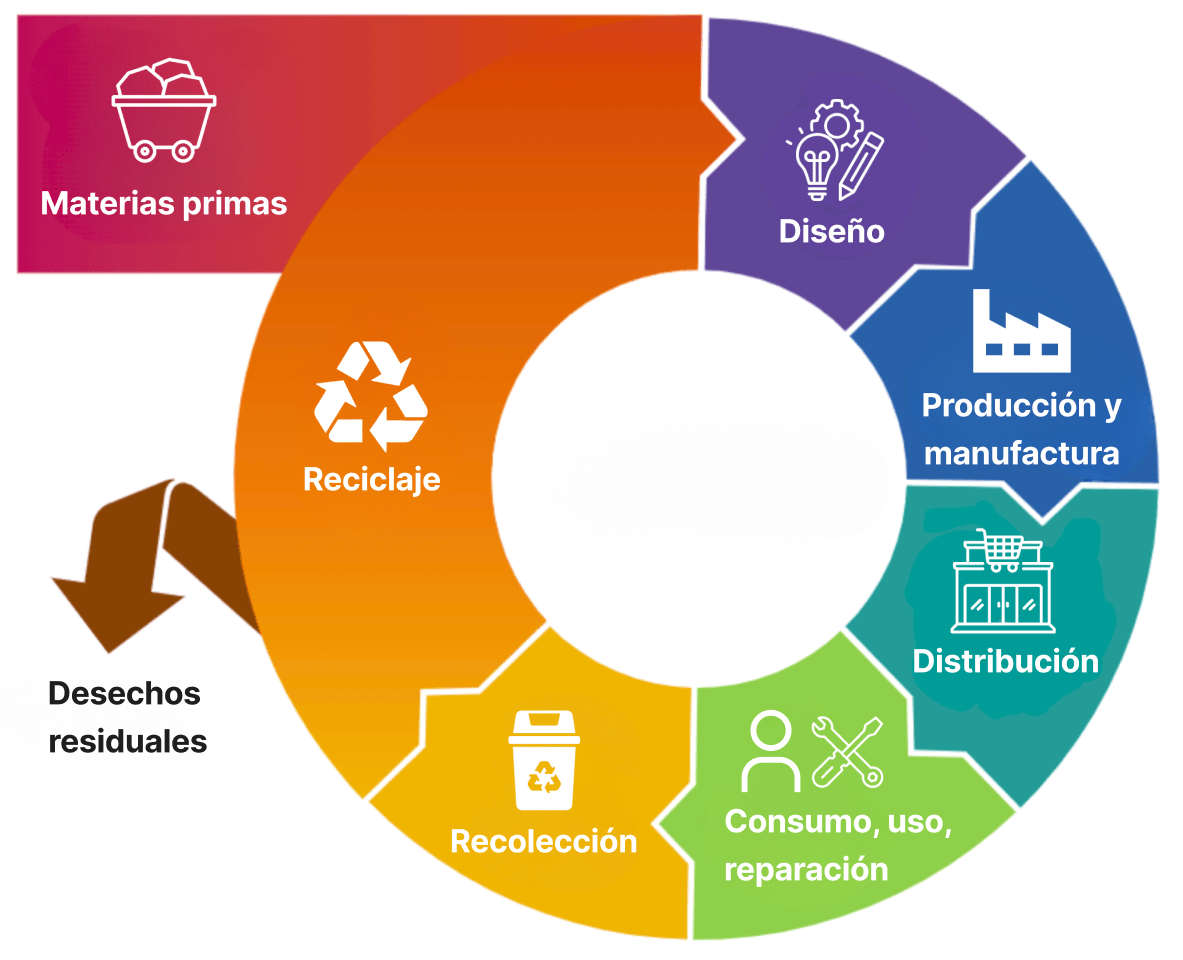
\includegraphics[width=0.8\textwidth]{Figures/circular-economy-stages.png}
    \caption{Ciclo productivo de la economía circular}
    \label{fig:circular-economy-stages}
\end{figure}

El proceso de producción comienza propiamente con la etapa de diseño, donde se decide la composición de los productos considerando criterios de ecoeficiencia, reutilización y reciclabilidad. Aquí intervienen diseñadores, ingenieros y proveedores de materias primas, quienes priorizan materiales reciclados o de bajo impacto ambiental. A continuación, durante la fabricación, los procesos industriales buscan reducir el uso de recursos y minimizar las emisiones, integrando tecnologías limpias y eficientes. En esta fase, los productos terminados o semielaborados quedan registrados con información detallada sobre su origen, composición y trazabilidad, lo cual permite una futura gestión más eficiente de su reciclaje. Tras su elaboración, los productos son distribuidos a través de canales logísticos que buscan optimizar los costos e impacto ambiental del transporte y almacenamiento.

Una vez que los productos son utilizados por los consumidores, comienza el ciclo inverso de valorización. Cuando estos artículos llegan al fin de su vida útil (y ya no pueden ser reutilizados), se convierten en residuos que deben ser recolectados, transportados, clasificados y reciclados o reacondicionados. Este proceso, conocido de forma genérica como "reciclaje" (sin distinguir si el destino final es reacondicionamiento o reciclaje), involucra a recolectores, centros de acopio, plantas de tratamiento, recicladores industriales y fabricantes secundarios. Durante la recolección, tecnologías como sensores IoT, lectores de códigos QR o etiquetas RFID permiten registrar información sobre la identidad del recolector, la cantidad, el tipo y las condiciones del residuo. Esta información permite monitorear flujos de materiales y brindar transparencia en la cadena. En el primer paso del proceso de reciclaje, los residuos son transportados a instalaciones donde se clasifican y segregan según su tipo y calidad. Este paso es fundamental para evitar contaminaciones cruzadas entre materiales distintos y asegurar un reciclaje efectivo. Posteriormnte, los materiales seleccionados se someten a procesos de reciclaje o reacondicionamiento, reincorporándolos al sistema productivo como insumos o productos reutilizables. En todo este proceso, tecnologías como blockchain pueden documentar cada transacción o transformación del material, documentando la integridad del proceso y fomentando la confianza entre los actores.

El esquema de la Figura \ref{fig:baralla-model-1} ilustra las distintas aplicaciones posibles de la tecnología blockchain en cada etapa del ciclo completo de economía circular. En este sistema ilustrado, la tecnología blockchain conecta las etapas en un flujo de información unificada, formando un sistema de trazabilidad digital que permite el seguimiento de los materiales desde su origen hasta su reincorporación al sistema o disposición final.

\begin{figure}[!htpb]
    \centering
    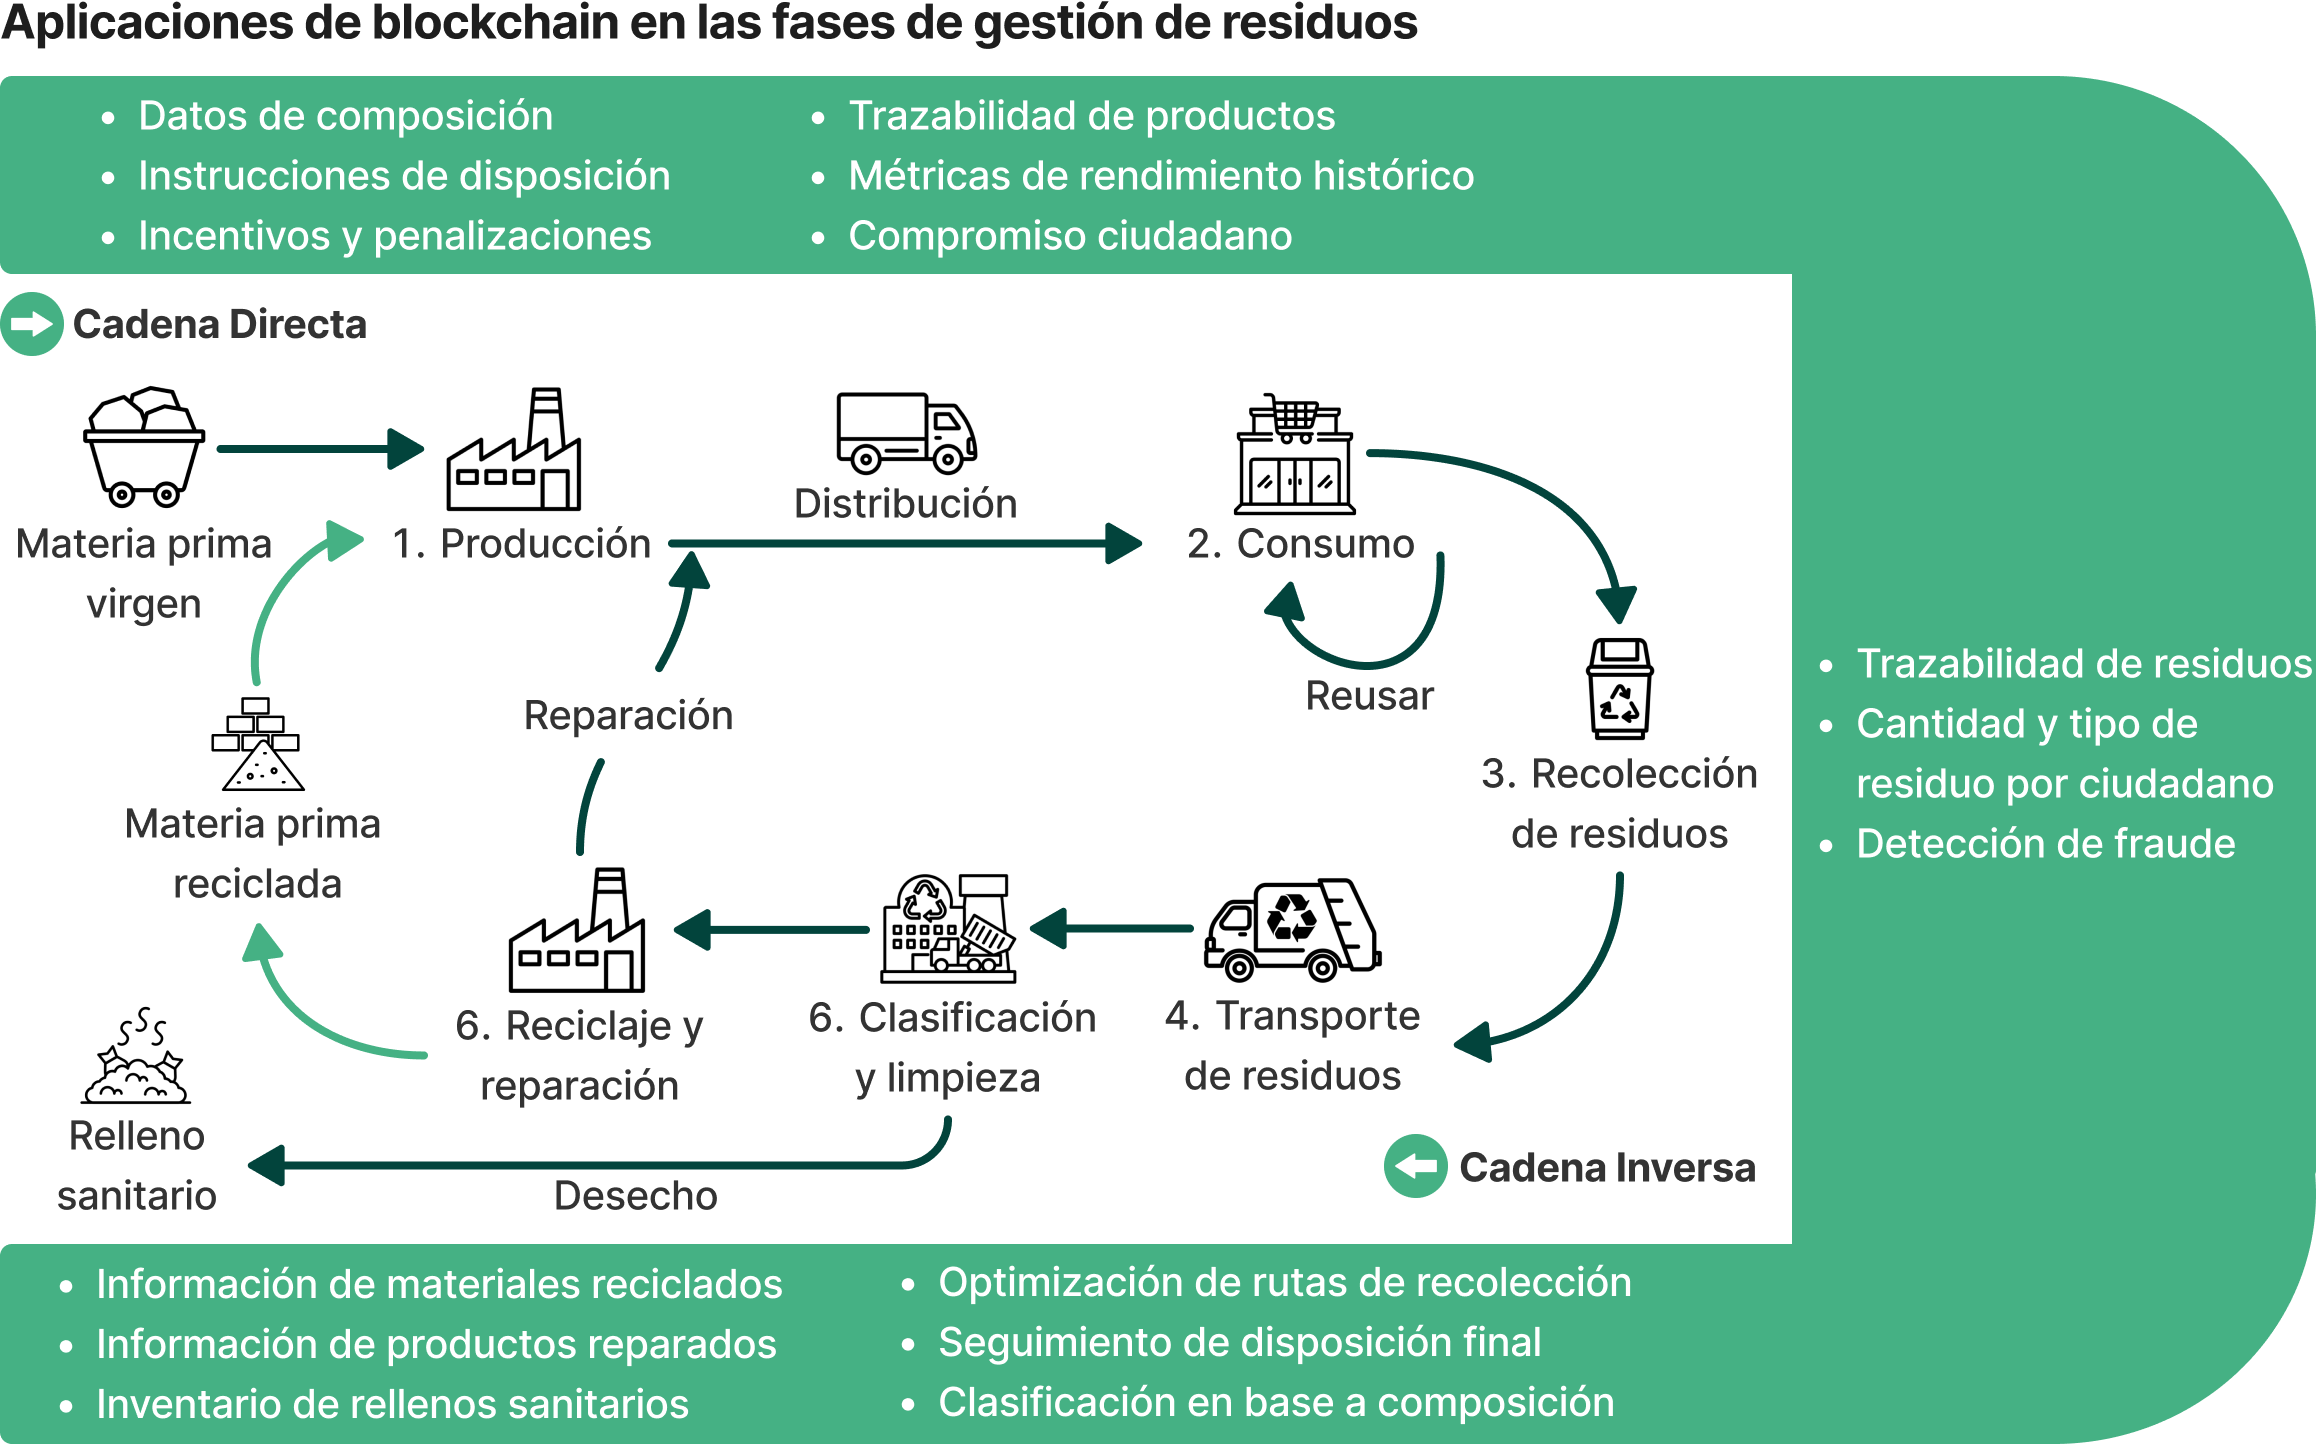
\includegraphics[width=0.8\textwidth]{Figures/baralla-model-1.png}
    \caption{Usos de la tecnología blockchain en las etapas de la economía circular \cite{baralla2023waste}}
    \label{fig:baralla-model-1}
\end{figure}

El proceso de reciclaje varía en complejidad dependiendo del material. Existen diversos materiales reciclables, cada uno con características particulares. El papel y cartón son ampliamente reciclados y fáciles de recolectar, mientras que los metales (como el aluminio, el acero o el cobre) conservan sus propiedades tras múltiples ciclos. Los residuos electrónicos presentan un alto valor por su contenido en metales preciosos, aunque requieren procesos especializados para su desmontaje. Los plásticos representan un desafío por su heterogeneidad, pero pueden reciclarse eficientemente si se rediseñan los envases y se simplifican sus composiciones. Los residuos orgánicos son compostables o pueden aprovecharse energéticamente en caso de no mezclarse con residuos no reciclables. Finalmente, el vidrio destaca como el material circular por excelencia: puede reciclarse infinitas veces sin perder calidad, su estructura es químicamente estable, y su reciclaje requiere menos energía que su producción original. Estas cualidades lo convierten en un insumo ideal para sistemas de economía circular bien diseñados.

\subsection{Cadena de suministro del vidrio}

El vidrio es uno de los materiales más representativos de la economía circular por su capacidad única de ser reciclado indefinidamente sin perder calidad. Esta propiedad lo convierte en un recurso estratégico para reducir la demanda de materias primas vírgenes, minimizar residuos y disminuir la huella de carbono asociada a la producción industrial. A diferencia de otros materiales cuyo reciclaje implica degradación, el vidrio conserva íntegramente sus características físicas y químicas, permitiendo su reintegración al ciclo productivo tantas veces como sea necesario. En la Figura \ref{fig:glass-lifecycle} se muestra el ciclo de vida del vidrio en un modelo de economía circular, que abarca desde la extracción de materias primas hasta su reincorporación como materia prima en nuevos productos, ejemplificando el caso de los envases de vidrio.

\begin{figure}[!htpb]
    \centering
    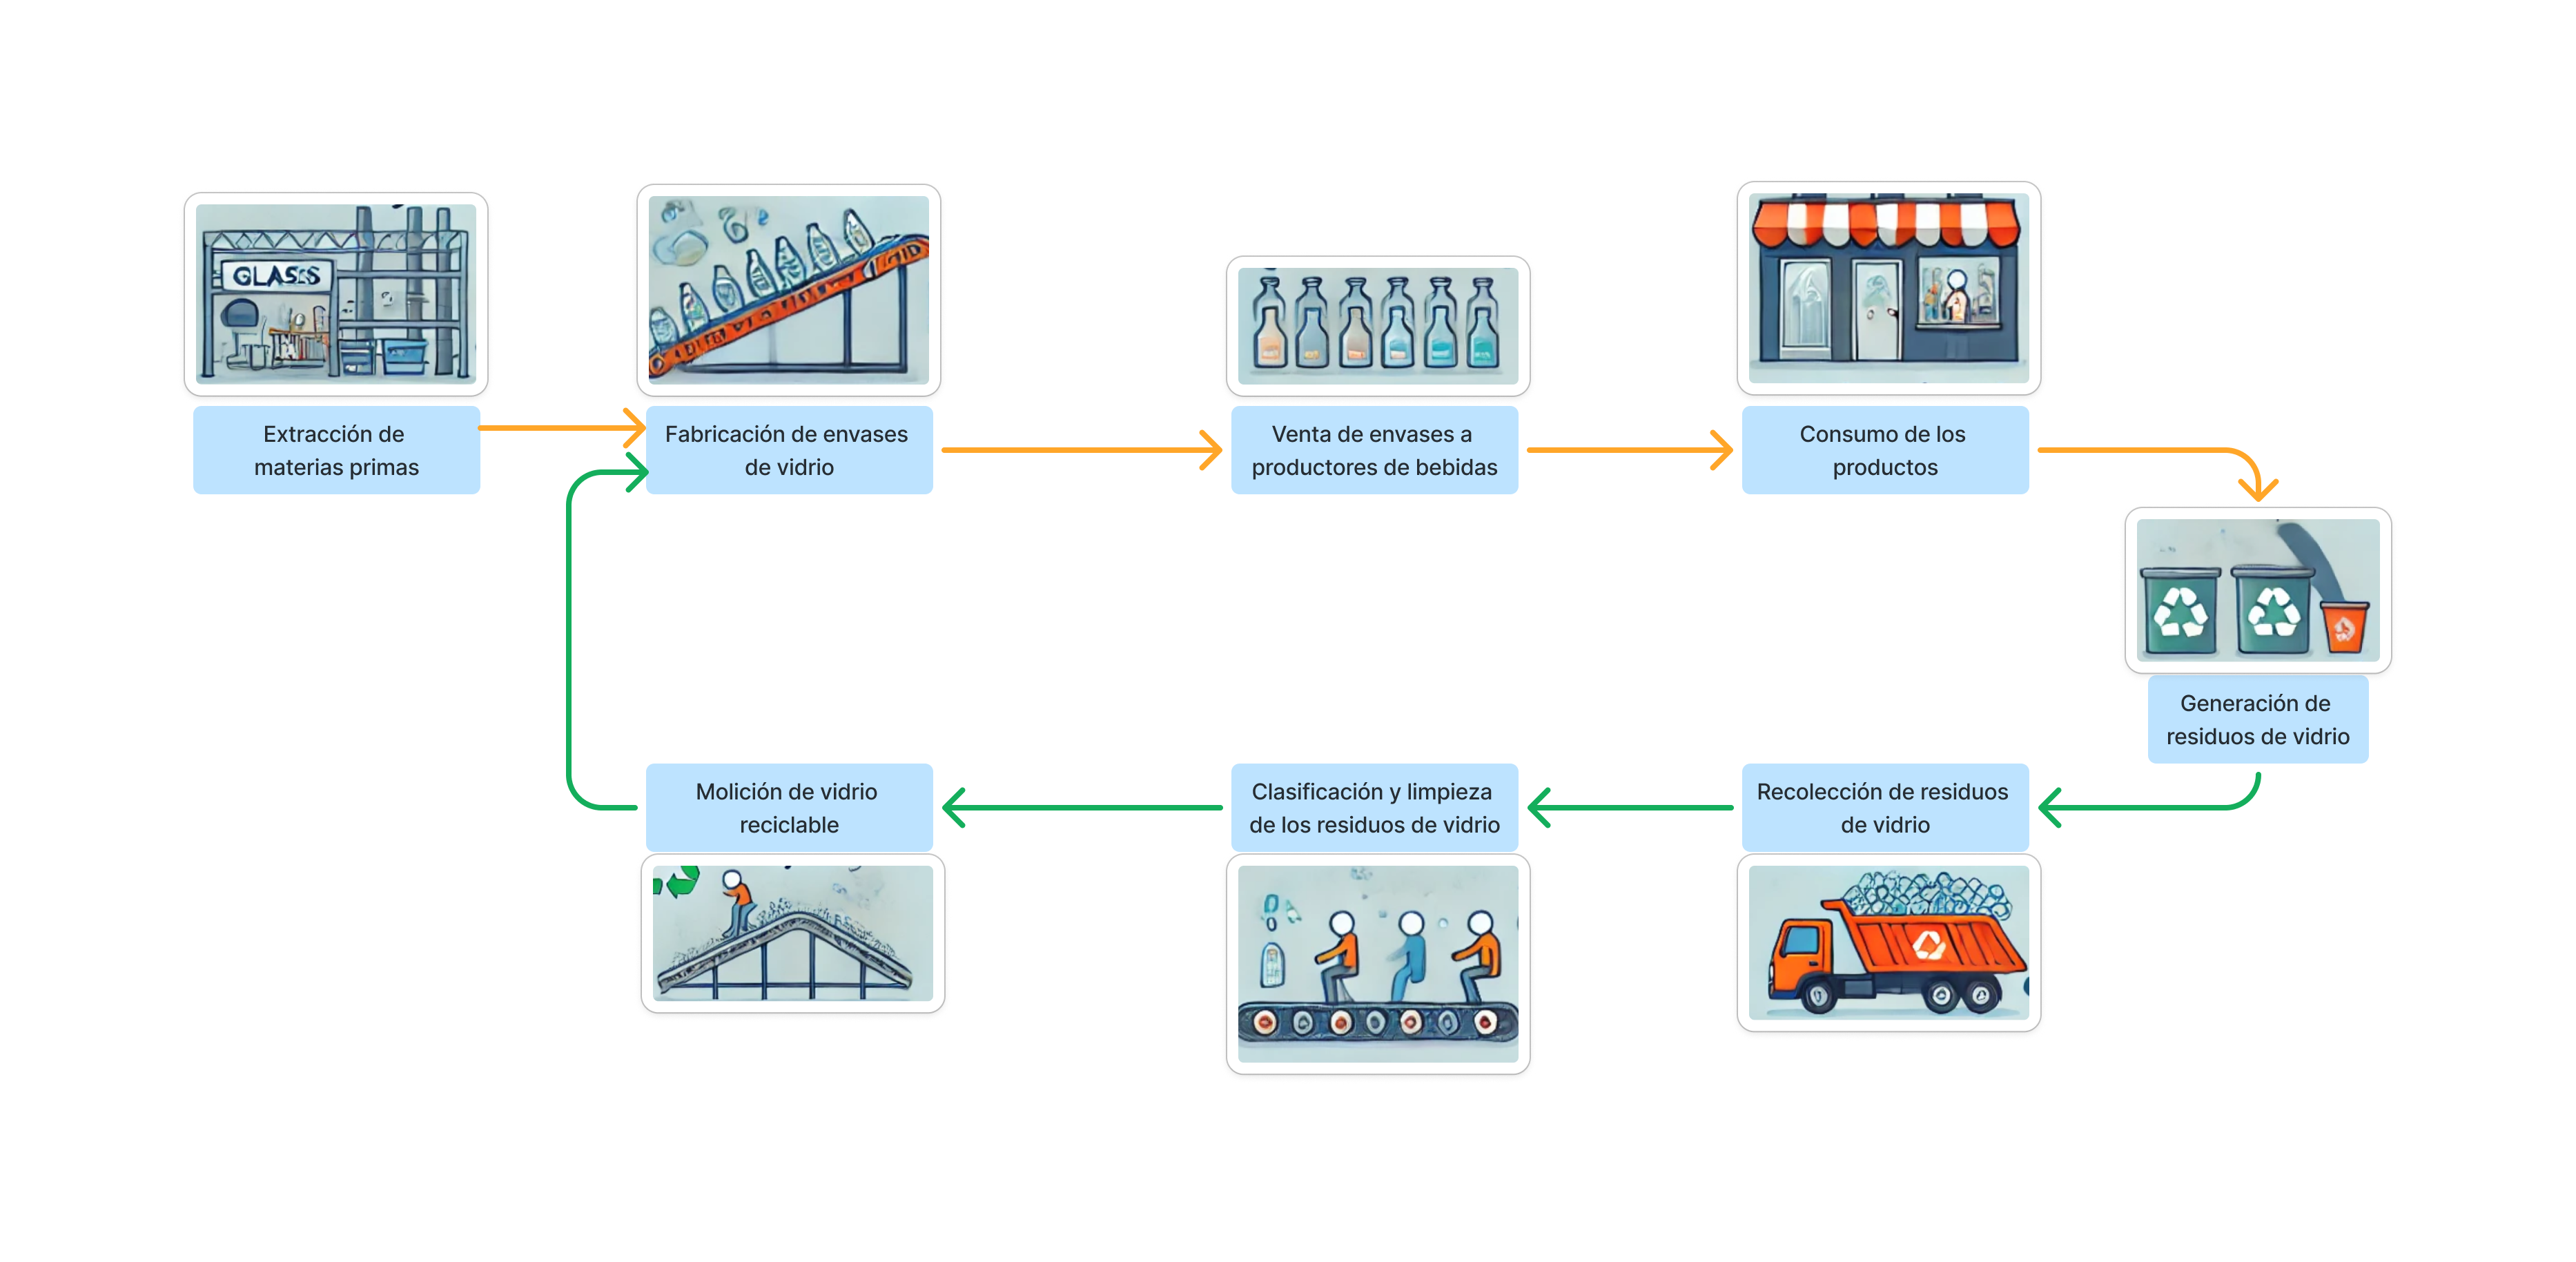
\includegraphics[width=0.8\textwidth]{Figures/glass-lifecycle.png}
    \caption{Ciclo de vida de envases de vidrio en un modelo de economía circular}
    \label{fig:glass-lifecycle}
\end{figure}

% TODO: consider rewriting this with verallia steps listing (tex/theoretical-framework.tex)

El proceso comienza con el diseño del producto, etapa clave para asegurar su durabilidad, reutilización y posterior reciclabilidad. Por ejemplo, en la producción de envases de vidrio, en esta etapa se deciden aspectos como color, forma y composición del envase para optimizar durabilidad, reciclabilidad y aspectos estéticos. Luego del diseño, sigue la producción industrial, donde se funden arena, sosa y caliza a altas temperaturas, frecuentemente combinadas con calcín (vidrio reciclado triturado) para reducir el consumo energético y demanda de materiales vírgenes. La especial reciclabilidad del vidrio se hace visible en esta etapa, ya que la calidad del vidrio resultante es la misma sin importar la proporción de calcín y de materiales vírgenes utilizados (característica que, por ejemplo, no es igual para el plástico), por lo que los productores de vidrio no encuentran pérdidas potenciales al utilizar materiales reciclados. Luego, los envases fabricados son distribuidos, utilizados para embotellar bebidas (por ejemplo, vino) y adquiridos por los consumidores, quienes (luego de consumir su contenido) pueden reutilizarlos, descartarlos (como basura común) o ingresarlos a circuitos de reciclaje. Para el correcto reciclaje del vidrio (y otros materiales) es importante el circuito de recolección diferenciada, que evita que el vidrio reciclable se mezcle con otros materiales que lo contaminen e imposibiliten su reciclaje. Los residuos de vidrio son recolectados por empresas especializadas o por los propios consumidores, quienes pueden depositarlos en contenedores específicos para su posterior tratamiento.
Una vez recolectado, el vidrio es transportado a plantas de reciclaje donde se clasifica. En la clasificación se separa al vidrio de otros materiales reciclables que puedan haber sido mezclados y se separan los distintos tipos de vidrio (por ejemplo, por color), ya que algunas características, como el color y la composición química, son relevantes para el posterior uso del vidrio reciclado. Luego, el vidrio es triturado y limpiado para eliminar impurezas, como etiquetas o restos de alimentos, dando como resultado lo que se conoce como calcín. Esta etapa es crucial, ya que la pureza del material reciclado influye directamente en la calidad del vidrio producido. Finalmente, el calcín se funde nuevamente y se convierte en materia prima para nuevos envases, cerrando así el ciclo de vida del vidrio. Este proceso de reciclaje puede repetirse indefinidamente, lo que lo convierte en un modelo ejemplar de economía circular.

La cadena de suministros y reciclaje de envases de vidrio tiene una importancia estratégica en la provincia de Mendoza, por su estrecha vinculación con la industria vitivinícola, uno de los principales motores económicos de la región. La provincia cuenta con una única empresa que produce y recicla envases de vidrio a escala industrial: Verallia. Esta compañía internacional cubre la totalidad de la demanda local de botellas y frascos, fabricando envases para vinos, espumantes, cervezas, licores y alimentos. El proceso de producción en Verallia incluye desde la selección y mezcla de materias primas hasta la formación, inspección y distribución de los envases, con la integración progresiva de vidrio reciclado como parte del insumo.

Verallia ha reconocido públicamente que la mayor dificultad de su industria es la elevada emisión de dióxido de carbono, por lo que ha adoptado una estrategia dual orientada a optimizar el reciclaje y fomentar la reutilización del vidrio. Bajo esta lógica, ha desarrollado el programa "Vidrio, una acción transparente" en alianza con el Gobierno de Mendoza, mediante el cual se promueve la recolección de envases descartados, destinando los ingresos generados al apoyo de organizaciones benéficas. Esta iniciativa, aunque aún incipiente, representa un esfuerzo por avanzar hacia una cadena de suministro más circular y socialmente responsable en la provincia.

Sin embargo, el reciclaje de vidrio en Mendoza enfrenta desafíos estructurales. La tasa de recuperación aún es baja, las métricas oficiales son escasas y las políticas de incentivo son limitadas. La logística de recolección depende en gran medida de la voluntad ciudadana y carece de sistemas obligatorios o premiantes que aseguren su masividad. En este contexto, el rol de actores industriales como Verallia resulta central para impulsar transformaciones sostenibles en la cadena del vidrio, tanto mediante la innovación tecnológica como a través de la articulación público-privada.

Más allá del caso mendocino, el vidrio sigue siendo uno de los materiales más valiosos dentro de una economía circular bien implementada. Su durabilidad, estabilidad química, transparencia y capacidad de reciclaje total lo convierten en un insumo ideal para cerrar ciclos productivos sin pérdidas de calidad ni de valor. Avanzar hacia una cadena del vidrio plenamente circular requiere optimizar cada etapa, desde el diseño y la fabricación hasta la trazabilidad del reciclaje, consolidando sistemas logísticos eficientes, ciudadanos comprometidos y políticas públicas robustas que garanticen su sostenibilidad a largo plazo. A continuación, se explorarán los proyectos y trabajos relacionados que han abordado la trazabilidad y el reciclaje de vidrio, así como otras iniciativas vinculadas a la economía circular y la sostenibilidad que plantean e implementan soluciones innovadoras para mejorar la gestión de residuos y fomentar prácticas responsables en la cadena de suministro.

\section{Proyectos y trabajos relacionados}

% TODO: fill this section with related projects and works

[Mencionar y describir de manera fluída algunos de todos estos proyectos, comenzando desde lo más simple a lo más complejo. Primero tecnología para incentivar reciclaje, luego uso de blockchain en cadena de suministros, luego específicamente orientado a sustentabilidad y por último que además se concentren en dar trazabilidad. Sacar en limpio los aportes relevantes de cada uno y los puntos débiles (que resolverá mi trabajo)].

Tecnología con incentivos para el reciclaje:
\begin{itemize}
    \item DRS (PFAND, Alemania)
    \item Reciclos (España)
    \item Colmena (Argentina)
    \item Greenly Points (Argentina)
    \item Plastic Bank (Canadá)
\end{itemize}

Aplicaciones de tecnología blockchain en la cadena de suministro para logística/trazabilidad:
\begin{itemize}
    \item Signeblock (España)
\end{itemize}

Uso de tecnología blockchain en la cadena de suministro para la sustentabilidad:
\begin{itemize}
    \item Modelo para la gestión de residuos [baralla2023waste]
    \item Modelo ZERO para el Reciclaje de Plásticos con Tecnología Blockchain
    \item Uso de Blockchain y Marcadores Moleculares para el Manejo Sostenible de Residuos Plásticos
\end{itemize}

Uso de tecnología blockchain en la cadena de suministro para trazabilidad para Sustentabilidad:
\begin{itemize}
    \item Circularise (Holanda)
    \item Circulor (Reino Unido)
\end{itemize}

[Debo cerrar de alguna manera con conclusión o un párrafo el marco teórico antes de saltar a metodología? Quizás contar dónde acotamos el problema vistos los proyectos preexistentes? Dónde cuento que elegimos vidrio en Mendoza por el vino y que vamos a hacer un sistema de trazabilidad específicamente para esa cadena de suministros y todos sus actores??]
